\documentclass[12pt,titlepage]{article}

\usepackage{fullpage}
\usepackage{amsmath}
\usepackage{makeidx}
\usepackage{epsfig}
\usepackage[hyperfootnotes=false]{hyperref}
\usepackage{longtable}
\usepackage[width=.85\textwidth]{caption}

\newcommand{\sub}[1]{\ensuremath{_{\mbox{\scriptsize \,#1}}}}
\newcommand{\supers}[1]{\ensuremath{^{\mbox{\scriptsize #1}}}}

\newcommand{\cname}[1]{\index{#1}\textsf{#1}}
\newcommand{\E}{\ensuremath{\mathbb{E}}}
\newcommand{\V}{\ensuremath{\mathbb{V}}}
\newcommand{\R}{\ensuremath{\mathbb{R}}}
\newcommand{\etal}{\emph{et al.}}
\newcommand{\hf}{\hat{f}_N}
\newcommand{\xf}{x\sub{fit}}
\newcommand{\scriptname}[1]{\texttt{#1}}
\newcommand{\at}{\tilde{a}\sub{fit}}
\newcommand{\bt}{\tilde{b}\sub{fit}}

\makeindex
\renewcommand\indexname{Functions and Classes}

\newenvironment{thinlist} {
    \begin{list} {---} {
        \setlength{\topsep}{0.075cm}
        \setlength{\parsep}{0.075cm}
        \setlength{\itemsep}{0.075cm}
    }
} {\end{list}}


\begin{document}

\title{Statistical Methods in the NPStat Package}
\author{I. Volobouev, {\it i.volobouev@ttu.edu}}
\date{Version: 4.9.0 \hspace{1.5cm} Date: \today}
\maketitle

\tableofcontents

\newpage
\section{Preliminaries}
\label{sec:preliminaries}

The NPStat package provides a C++ implementation of 
several nonparametric
statistical modeling tools together with
various supporting code. Nonparametric modeling becomes very
useful when there is little prior information available to justify an
assumption that the data belongs to a certain parametric family of
distributions. Even though nonparametric techniques are usually
more computationally intensive than parametric ones,
judicious use of fast algorithms in combination with
increasing power of modern computers often results in very practical
solutions --- at least until the ``curse of dimensionality'' starts
imposing its heavy toll.

It will be assumed that the reader of this note is reasonably
proficient in C++ programming, and that the meaning
of such words as ``class'', ``function'', ``template'',
``method'', ``container'', ``namespace'', {\it etc.}
is obvious from their context.

The latest version of the package code can be downloaded from
\href{http://npstat.hepforge.org/}{http://npstat.hepforge.org/}
Most classes and functions implemented in NPStat are placed in the 
``npstat'' namespace. A~few functions and classes that
need Minuit2~\cite{ref:minuit} installation
in order to be meaningfully used belong
to the ``npsi'' namespace. Such functions and
classes can be found in the ``interfaces''
directory of the package.

When a C++ function, class, or template is mentioned in the text
for the first time, the header file which contains its declaration
is often mentioned as well. If the header file is not mentioned,
it is most likely ``npstat/stat/NNNN.hh'', where NNNN stands
for the actual name of the class or function.

An expression ``$I(Q)$'' is frequently employed in the text,
where $Q$ is some logical proposition.
$I(Q)$ is the proposition indicator function
defined as follows: $I(Q) = 1$ if $Q$ is true
and $I(Q) = 0$ if $Q$ is false. For example, a product of $I(0 \le x \le 1)$
with some other mathematical function is often used to
denote some probability density supported
on the $[0, 1]$ interval. Note that $I(\neg Q) = 1 - I(Q)$, where 
$\neg Q$ is the logical negation of $Q$. 


\section{Data Representation}
\label{sec:datarep}

For data storage, the NPStat software relies on the object serialization
and I/O capabilities provided
by the C++ Geners package~\cite{ref:geners}.
Geners supports persistence of all standard library containers
(vectors, lists, maps, {\it etc.}) including those introduced
in the C++11 Standard~\cite{ref:cpp11} (arrays, tuples, unordered sets
and maps). In addition to data structures supported by Geners, NPStat
offers several other persistent containers useful in statistical
data analysis: multidimensional arrays, homogeneous $n$-tuples, and
histograms.

Persistent multidimensional arrays are implemented with the \cname{ArrayND}
template (header file ``npstat/nm/ArrayND.hh'').
This is a~reasonably full-featured array class, with support for
subscripting (with and without bounds checking), vector space operations
(addition, subtraction,
multiplication by a scalar), certain tensor operations (index contraction,
outer product), slicing, iteration over subranges, linear and cubic
interpolation of array values
to fractional indices, {\it etc.} Arrays whose maximum
number of elements is known at the compile time can be efficiently
created on the stack.

Homogeneous $n$-tuples are two-dimensional tables in which the number of
columns is fixed while the number of rows can grow dynamically.
The stored object type is chosen when the $n$-tuple is created
(it is a template parameter). For
homogeneous $n$-tuples, storage type is the same for every column
which allows for more efficient optimization of memory allocation
in comparison with heterogeneous $n$-tuples.\footnote{The Geners
serialization package supports
several types of persistent heterogeneous $n$-tuples including
std::vector$<$std::tuple$<$...$> >$, 
RowPacker variadic template
optimized for accessing large data samples row-by-row,
and ColumnPacker variadic template
optimized for data access column-by-column.}
Two persistent template classes are provided for homogeneous $n$-tuples:
\cname{InMemoryNtuple} for $n$-tuples which can completely fit inside
the computer memory (header file ``npstat/stat/InMemoryNtuple.hh'')
and \cname{ArchivedNtuple} for $n$-tuples
which can grow as large as the available disk space
(header file ``npstat/stat/ArchivedNtuple.hh''). Both of these
classes inherit from the abstract class \cname{AbsNtuple} which
defines all interfaces relevant for statistical analysis of the data
these $n$-tuples contain. Thus \cname{InMemoryNtuple} and \cname{ArchivedNtuple}
are completely interchangeable for use in various data analysis algorithms.

Arbitrary-dimensional\footnote{To be precise,
the number of dimensions for both histograms
and multidimensional arrays can not exceed
31 on 32-bit systems and 63 on 64-bit systems. However, your computer will
probably run out of memory long before this limitation
becomes relevant for your data analysis.} persistent
histograms are implemented with the \cname{HistoND}
template (header file ``npstat/stat/HistoND.hh''). Both uniform and non-uniform
placing of bin edges can be created using
axis classes \cname{HistoAxis} and \cname{NUHistoAxis}, respectively,
as \cname{HistoND} template parameters. The \cname{DualHistoAxis} class
can be employed for histograms in which only a fraction of axes
must have non-uniform bins.
Two binning schemes are supported
for data sample processing.
In the normal scheme, the bin count is incremented if the point coordinates
fall inside the given bin (the \cname{fill} method of the class).
In the centroid-preserving scheme,
all bins in the neighborhood of the sample point
are incremented in such a way that the center of mass of bin
increments coincides exactly with the point location
(the \cname{fillC} method)\footnote{For one-dimensional histograms,
this is called ``linear binning''~\cite{ref:linearbinning}.
NPStat supports this technique for uniformly binned
histograms of arbitrary dimensionality.}.
The objects used as
histogram bin contents and the objects used as
weights added to the bins when
the histogram is filled are not required to have
anything in common; the only requirement is that a~meaningful
binary function (typically, operator+=) can be defined for them.
This level of abstraction allows, for example, for using vectors and tensors
as histogram bin contents or for implementing profile histograms with
the same \cname{HistoND} template. As the bin contents are implemented
with the \cname{ArrayND} class, all features of \cname{ArrayND}
(vector space operations, slicing, interpolation, {\it etc}) are available
for them as well. Overflows are stored in separate arrays with
three cells in each dimension: underflow, overflow, and the central part
covered by the regular histogram bins.

\section{Descriptive Statistics}
\label{sec:descriptivestats}

A number of facilities is included in the NPStat package for calculating
standard descriptive sample statistics such as mean, covariance matrix,
{\it etc}. Relevant functions, classes, and templates are described below.

\subsection{Functions and Classes for Use with Point Clouds}

\cname{arrayStats} (header file ``npstat/stat/arrayStats.hh'') --- This
function estimates the population mean ($\mu$), standard deviation ($\sigma$),
skewness ($s$),
and kurtosis ($k$) for a one-dimensional set of points. A numerically sound
two-pass algorithm is used.
% Internally, calculations are performed in long double precision. 
The following formulae are implemented ($N$ is the number of points
in the sample):
\begin{equation}
\mu = \frac{1}{N} \sum_{i=0}^{N-1} x_i
\label{eq:samplemean}
\end{equation}
\begin{equation}
\sigma = \sqrt{\frac{1}{N - 1} \sum_{i=0}^{N-1} (x_i - \mu)^2}
\label{eq:samplestdev}
\end{equation}
\begin{equation}
s = \frac{N}{(N - 1) (N - 2) \sigma^3} \sum_{i=0}^{N-1} (x_i - \mu)^3
\end{equation}
\begin{equation}
g_2 = N \frac{\sum_{i=0}^{N-1} (x_i - \mu)^4}{\left( \sum_{i=0}^{N-1} (x_i - \mu)^2 \right)^2} - 3
\label{eq:kurtosisg2}
\end{equation}
\begin{equation}
k = \frac{N - 1}{(N - 2) (N - 3)} ((N + 1) g_2 + 6) + 3
\label{eq:kurtosis}
\end{equation}
Note that the population kurtosis estimate is defined in such a way that its
expectation value for a sample drawn from the Gaussian distribution equals
3 rather than 0. For more details on the origin of these formulae
consult Ref.~\cite{ref:sampleskewkurt}.

\cname{empiricalCdf} (header file ``npstat/stat/StatUtils.hh'') --- This
function evaluates the empirical cumulative distribution function (ECDF) for
a sample of points. The points must be sorted
in the increasing order  by the user before
the function call is made.
The ECDF is defined as follows. Suppose, the $N$ sorted point values are
$\{x_0, x_1, ..., x_{N-1}\}$ and all $x_i$ are distinct ({\it i.e.,} there
are no ties). Then
\begin{equation}
\mbox{ECDF}(x) = \left\{ \begin{array}{ll}
                         0 & \mbox{if\ } x \le x_0, \\
                         \frac{1}{N} \left( \frac{x-x_i}{x_{i+1}-x_i}+i+1/2 \right) & \mbox{if\ } x_i < x \le x_{i+1} \ \mbox{and} \ x < x_{N-1}, \\
                         1 & \mbox{if\ } x \ge x_{N-1}.
                         \end{array}
                 \right.
\label{eq:ecdf}
\end{equation}
When all sample points are distinct, $\mbox{ECDF}(x)$ is discontinuous
at $x = x_0$ and $x = x_{N-1}$ and continuous for all other $x$.
If the sample has more than one point
with the same $x$, let say $x_k$ and
$x_{k+1}$ where $k > 0$ and $k < N - 2$, $x_k$ also becomes
a point of discontinuity.
$\mbox{ECDF}(x_k)$ will be set to $\frac{1}{N} (k + 1/2)$, the value
coincident with the function left limit.

\cname{empiricalQuantile} (header file ``npstat/stat/StatUtils.hh'') --- This
is the empirical quantile function, $\mbox{EQF}(y)$, which provides
an inverse to $\mbox{ECDF}(x)$. For any $x$ from the interval
$[x_0, x_{N-1}]$, $\mbox{EQF}(\mbox{ECDF}(x)) = x$ (up to numerical
round-off errors). If $x < x_0$ then $\mbox{EQF}(\mbox{ECDF}(x)) = x_0$ and if
$x > x_{N-1}$ then $\mbox{EQF}(\mbox{ECDF}(x)) = x_{N-1}$.

\cname{MultivariateSumAccumulator} and \cname{MultivariateSumsqAccumulator}
--- These classes are intended for calculating means and covariance matrices
    for multivariate data samples in a~numerically stable manner. The
    classes can be
    used inside user-implemented cycles over sets of points or with
    \cname{cycleOverRows} and other similar methods of the \cname{AbsNtuple}
    class. Two passes over the data
    are necessary for calculating the covariance matrix,
    first with
    \cname{MultivariateSumAccumulator} and second with
    \cname{MultivariateSumsqAccumulator}. The multivariate
    mean is initially found from
\begin{equation}
\overline{{\bf x}} = \frac{1}{N} \sum_{i=0}^{N-1} {\bf x}_i
\end{equation}
and then an estimate of the population covariance matrix is calculated as
\begin{equation}
V = \frac{1}{N - 1} \ 
    \sum_{i=0}^{N-1} ({\bf x}_i - \overline{{\bf x}}) ({\bf x}_i - \overline{{\bf x}})^T
\label{eq:covar}
\end{equation}

\cname{MultivariateWeightedSumAccumulator} and
\cname{MultivariateWeightedSumsqAccumulator} --- These classes are
intended for calculating means and covariance matrices
for multivariate data samples in which points enter with non-negative
weights:
\begin{equation}
\overline{{\bf x}} = \frac{\sum_{i=0}^{N-1} w_i {\bf x}_i}{\sum_{i=0}^{N-1} w_i},
\label{eq:weightedmean}
\end{equation}
\begin{equation}
V = \frac{N_{eff}}{N_{eff} - 1} \ 
    \frac{\sum_{i=0}^{N-1} w_i ({\bf x}_i - \overline{\bf x}) ({\bf x}_i - \overline{\bf x})^T}{\sum_{i=0}^{N-1} w_i},
\label{eq:weightedcov}
\end{equation}
where $N_{eff}$ is the effective number of entries in a weighted
sample\footnote{$N_{eff}$ is also known as the Kish's effective sample size. Note that this
estimate of $V$ makes sense only if the weights and point locations are statistically independent
from each other. If the weights are functions of the observed ${\bf x}_i$ then there
appears to be no general estimate that is independent of the weighting function.}:
\begin{equation}
N_{eff} = \frac{\left( \sum_{i=0}^{N-1} w_i \right)^2}{\sum_{i=0}^{N-1} w_i^2}.
\label{eq:neff}
\end{equation}
Two passes over the data are required, first with
\cname{MultivariateWeightedSumAccumulator} and then with
\cname{MultivariateWeightedSumsqAccumulator}.

\cname{StatAccumulator} --- Persistent class which determines
the minimum, the maximum, the mean, and the standard
deviation of a~sample of values using a single-pass algorithm.
It can be used when the two-pass calculation
is either impossible or impractical for
some reason. This class can be conveniently employed as
a bin content type for \cname{HistoND} (this turns \cname{HistoND}
into a profile histogram).
\cname{StatAccumulator}
maintains a running average which is updated
after accumulating $2^K$ points, $K = 0, 1, 2, ...$ The 
numerical precision of the standard deviation determined
in this manner is not as good as in the two-pass method but it
is usually much better than that expected
from a~naive implementation which simply accumulates sample moments about 0
and then evaluates $\sigma^2$ according to
$\frac{N}{N - 1} (\overline{{\bf x}^2} - {\overline{\bf x}}^2)$ (this formula
can suffer from a severe subtractive cancellation problem).

\cname{WeightedStatAccumulator} --- Similar class for calculating
mean and standard deviation of a~sample of weighted values using
a single-pass algorithm.

\cname{StatAccumulatorArr} --- This class provides functionality similar
to an array of \cname{StatAccumulator} objects but with a more convenient
interface for accumulating sample values (cycling over the input values
is performed by the class itself).

\cname{StatAccumulatorPair} --- Two \cname{StatAccumulator} objects
augmented by the sum of cross terms which allows for subsequent
calculation of covariance. The covariance is estimated using
a formula which can potentially suffer from subtractive
cancellation\footnote{This problem is partially alleviated
by using long double type for internal calculations.}.
Therefore, this class should not be used to process large samples of points in
which, for one of the variables or for both of them,
the absolute value of the mean can be much larger than the
standard deviation. This class is persistent.

\cname{CrossCovarianceAccumulator} --- To accumulate the sums for
covariance matrix calculation according to formula~\ref{eq:covar}
in $d$-dimensional space,
one has to keep track of $d (d + 1)/2$ sums of squares and cross terms.
Sometimes only a small part of the complete covariance matrix is of interest.
In this case $d$ can often be split into subspaces of dimensionalities
$d_1$ and $d_2$, $d = d_1 + d_2$, so that the interesting part of
covariance matrix is dimensioned $d_1 \times d_2$ (plus $d$ diagonal terms).
For large values
of $d$, accumulating $d + d_1 \times d_2$ sums instead of $d (d + 1)/2$
can mean big difference in speed and memory consumption, especially
in case $d_1 \ll d_2$ (or $d_1 \gg d_2$).
The \cname{CrossCovarianceAccumulator} allows
its users to do just that: it accumulates cross terms between two
arrays with $d_1$ and $d_2$ elements but not the cross terms between
elements of the same array. The covariances are estimated by a single-pass
method using a~formula which can suffer from subtractive
cancellation\footnotemark[5]. Use with care.

\cname{SampleAccumulator} --- This class stores all values
it gets in an internal buffer. Whenever mean, standard deviation,
or some quantile function values are needed for the accumulated sample,
they are calculated from the stored values using numerically sound techniques.
Mean and standard deviation are calculated according to
Eqs.~\ref{eq:samplemean} and~\ref{eq:samplestdev}.
Covariance and correlations can be calculated for a pair of
\cname{SampleAccumulator} objects with the same number of stored elements
by corresponding methods of the class.
Empirical CDF and empirical quantile calculations
are handled by calling \cname{empiricalCdf} and \cname{empiricalQuantile}
functions internally, preceded by data sorting.
This class is persistent and can be used as the bin content template
parameter for \cname{HistoND}.

\cname{WeightedSampleAccumulator} --- Similar to SampleAccumulator,
but intended for calculating various statistics for samples
of weighted points.

Kendall's $\tau$ and Spearman's $\rho$
rank correlation coefficients can be estimated
by functions \cname{sampleKendallsTau} and \cname{sampleSpearmansRho},
respectively. These functions are declared in the header files
``npstat/stat/kendallsTau.hh'' and ``npstat/stat/spearmansRho.hh'',
respectively.


\subsection{Functions for Use with Binned Data}

\cname{histoMean} (header file ``npstat/stat/histoStats.hh'') --- This
function calculates the histogram center of mass according to
Eq.~\ref{eq:weightedmean} with bin contents
used as weights for bin center coordinates.
Note that the code of this function does not enforce non-negativity of all bin
values, and the result of~\ref{eq:weightedmean} will not necessarily
make a lot of sense in case negative weights are present.
In order to check that all bins are non-negative
and that there is at least one positive bin, you can call the \cname{isDensity}
method of the \cname{ArrayND} class on the histogram
bin contents. The \cname{histoMean}
function is standalone and not a member of the \cname{HistoND} class
because Eq.~\ref{eq:weightedmean} is not going to make sense for all
possible bin types.

\cname{histoCovariance} (header file ``npstat/stat/histoStats.hh'') --- This
function estimates the population covariance matrix for histogrammed data
according to Eq.~\ref{eq:weightedcov}, with bin contents
used as weights for bin center coordinates.
As for \cname{histoMean}, results
produced by \cname{histoCovariance}
will not make much sense in case negative bin values are present.

\cname{arrayCoordMean} (header file ``npstat/stat/arrayStats.hh'') --- Similar
to \cname{histoMean} but the bin values are provided in an \cname{ArrayND}
object and bin locations are specified by additional arguments. 
Only uniform bin spacing is supported by this function
(unlike \cname{histoMean} which simply gets its bin centers from
the argument histogram).

\cname{arrayCoordCovariance} (header file ``npstat/stat/arrayStats.hh'') 
--- Similar to \cname{histoCovariance} but the bin values are provided
in an \cname{ArrayND} object and bin locations are specified by additional
arguments. Uniform binning only.

\cname{arrayShape1D} (header file ``npstat/stat/arrayStats.hh'') --- Estimates
population mean, standard deviation, skewness, and kurtosis for 
one-dimensional histogrammed data with equidistant bins.
Bin values $b_i$ used as weights are provided in an \cname{ArrayND}
object and bin locations $x_i$ are specified by additional arguments.
The mean and the standard deviations squared
are calculated according to Eqs.~\ref{eq:weightedmean}
and~\ref{eq:weightedcov} reduced to one dimension.
The skewness is estimated as
\begin{equation}
s = \frac{N_{eff}^2}{(N_{eff} - 1) (N_{eff} - 2) \sigma^3} \ 
\frac{\sum_{i=0}^{N_b-1} b_i (x_i - \mu)^3}{\sum_{i=0}^{N_b-1} b_i},
\end{equation}
with $N_{eff}$ defined by Eq.~\ref{eq:neff}. The kurtosis is found from Eq.~\ref{eq:kurtosis} in which $N$
is replaced by $N_{eff}$ and, instead of Eq.~\ref{eq:kurtosisg2},
$g_2$ is determined from
\begin{equation}
g_2 = \sum_{i=0}^{N_b-1} b_i \ \frac{\sum_{i=0}^{N_b-1} b_i (x_i - \mu)^4}{\left( \sum_{i=0}^{N_b-1} b_i (x_i - \mu)^2 \right)^2} - 3.
\end{equation}

\cname{arrayQuantiles1D} (header file ``npstat/stat/arrayStats.hh'')
--- This function treats
one-dimensional arrays as histograms and determines the values
of the quantile function for a~given set of cumulative density values
(after normalizing the histogram area to 1). Each bin is considered
to have uniform probability density between its edges. If you need
to perform this type of calculation more than once with the same
array, it will be more efficient to construct a \cname{BinnedDensity1D}
object and then to use its \cname{quantile} method instead of calling
the \cname{arrayQuantiles1D} function multiple times.

\cname{arrayEntropy} (header file ``npstat/stat/arrayStats.hh'')
--- This function calculates 
\begin{equation}
\label{eq:entropy}
H = -\frac{1}{N_b} \sum_{i=0}^{N_b-1} b_i \ln b_i
\end{equation}
This formula is appropriate for arrays that tabulate probability density
values on uniform grids. To convert the result  into the actual entropy
of the density, multiply it by the volume of the distribution support.


\subsection{ArrayND Projections}

The following set of classes works with \cname{ArrayND} class
and assists in making array ``projections''. 
Projections reduce array dimensionality
by calculating certain array properties over projected indices.
For example, one might want to create a one-dimensional array, $a$,
from a three-dimensional array, $b$, by summing all array elements
with the given second index: $a_j = \sum_{i, k} b_{ijk}$ (this means
that the first and the third indices of the array are ``projected''). This
and other similar operations can be performed by the \cname{project}
method of the \cname{ArrayND} class. What is done with the
array elements when the projection is performed can be specified
by the ``projector'' argument of the \cname{project} method. In particular,
this argument can be an object which performs some statistical
analysis of the projected elements.

\cname{ArrayMaxProjector} (header file ``npstat/stat/ArrayProjectors.hh'')
--- For each value of the array indices which are not projected,
    finds the maximum array element for all possible values of
    projected indices.

\cname{ArrayMinProjector} (header file ``npstat/stat/ArrayProjectors.hh'')
--- Finds the minimum array element for all possible values of
    projected indices.

\cname{ArraySumProjector} (header file ``npstat/stat/ArrayProjectors.hh'')
--- Sums all array values in the iteration over projected indices.

\cname{ArrayMeanProjector} (header file ``npstat/stat/ArrayProjectors.hh'')
--- Calculates the mean array value over projected indices.

\cname{ArrayMedianProjector} (header file ``npstat/stat/ArrayProjectors.hh'')
--- Calculates the median array value over projected indices.

\cname{ArrayStdevProjector} (header file ``npstat/stat/ArrayProjectors.hh'')
--- Calculates the standard deviation of array values encountered
    during the iteration over projected indices.

\cname{ArrayRangeProjector} (header file ``npstat/stat/ArrayProjectors.hh'')
--- Calculates the ``range'' of array values over projected indices.
    ``Range'' is defined here as the difference between 75\supers{th} and
    25\supers{th} percentiles of the sample values divided by the
    distance between 75\supers{th} and 25\supers{th} percentiles of
    the Gaussian distribution with $\sigma = 1$. Therefore, ``range'' can
    be used as a robust estimate of the standard deviation.

All ``projectors'' are derived either from \cname{AbsArrayProjector} class
in case the calculated quantity depends on the array indices
(header file ``npstat/nm/AbsArrayProjector.hh'')
or from \cname{AbsVisitor} class in case it is sufficient
to know just the element values (header file ``npstat/nm/AbsVisitor.hh'').
Naturally, the user
can supply his/her own projector implementations derived
from these base classes for use
with the the \cname{project} method of the \cname{ArrayND} class.


\section{Statistical Distributions}
\label{sec:distros}

A number of univariate and multivariate statistical distributions
is supported by the NPStat package. All implementations of
univariate continuous distributions share a common interface and can be
used interchangeably in a variety of statistical algorithms.
A similar approach has been adopted for univariate discrete and
multivariate continuous distributions.

\subsection{Univariate Continuous Distributions}

All classes which represent univariate continuous distributions
inherit from the \cname{AbsDistribution1D} abstract base class. These classes
must implement methods \cname{density} (probability density function),
\cname{cdf} (cumulative distribution function), \cname{exceedance}
(exceedance probability is just 1 $-$ cdf, but direct application
of this formula is often
unacceptable in numerical calculations due to subtractive cancellation),
and \cname{quantile} (the quantile function, inverse of cdf). For
a large number of statistical distributions, the probability density
function looks like $\frac{1}{\sigma}\, p\left( \frac{x - \mu}{\sigma} \right)$, where
$\mu$ and $\sigma$ are the distribution location and scale parameters, respectively.
Distributions of this kind should inherit from the base class 
\cname{AbsScalableDistribution1D} which handles proper
scaling and shifting of the argument (this base class itself inherits
from \cname{AbsDistribution1D}, and it is declared in the same
header file ``npstat/stat/AbsDistribution1D.hh'').

Some of the standard univariate continuous distributions implemented
in NPStat are listed in Table~\ref{table:distros1d}. A few special
distributions less frequently encountered in the statistical
literature are described in more detail in the following subsections.
Of course, user-developed classes inheriting from \cname{AbsDistribution1D}
or \cname{AbsScalableDistribution1D} can also be employed with all
NPStat functions and classes that take an instance of
\cname{AbsDistribution1D} as one of parameters.
\begin{longtable}{|c|c|c|}
% \captionsetup{width=.9\textwidth}
\caption{Continuous univariate distributions included in NPStat.
$P_n(x)$ are the Legendre polynomials.
Parameters $\mu$ and $\sigma$ are not shown for scalable distributions.
When not given explicitly, the normalization constant $\cal{N}$
ensures that 
$\int_{-\infty}^{\infty} p(x) dx = 1$. Most of the classes
listed in this table are declared in the header file
``npstat/stat/Distributions1D.hh''. If the distribution
is not declared in that header then it has a dedicated header
with the same name, {\it e.g.}, ``npstat/stat/TruncatedDistribution1D.hh''
for \cname{TruncatedDistribution1D}.}
\label{table:distros1d} \\

\hline \multicolumn{1}{|c|}{Class Name} &
\multicolumn{1}{c|}{$p(x)$} &
\multicolumn{1}{c|}{Scalable?} \\ \hline \hline 
\endfirsthead

\multicolumn{3}{c}%
{\tablename\ \thetable{} --- continued from the previous page} \\
\hline \multicolumn{1}{|c|}{Class Name} &
\multicolumn{1}{c|}{$p(x)$} &
\multicolumn{1}{c|}{Scalable?} \\ \hline \hline 
\endhead

\multicolumn{3}{|r|}{{Continued on the next page}} \\ \hline
\endfoot

\hline
\endlastfoot

\cname{Uniform1D} & $I(0 \le x \le 1)$ & yes \\ \hline
\cname{IsoscelesTriangle1D} & $(1 - |x|) I(-1 \le x \le 1)$ & yes \\ \hline
\cname{Exponential1D} & $e^{-x} I(x \ge 0)$ & yes \\ \hline
\cname{Quadratic1D} & $(1 + a P_1(2 x - 1) + b P_2(2 x - 1)) \,I(0 \le x \le 1)$ & yes \\ \hline
\cname{LogQuadratic1D} & ${\cal{N}} \exp (a P_1(2 x - 1) + b P_2(2 x - 1)) \,I(0 \le x \le 1)$ & yes \\ \hline
\cname{Gauss1D} & $\frac{1}{\sqrt{2 \pi}} e^{-x^2/2}$ & yes \\ \hline
\cname{GaussianMixture1D} & $\frac{1}{\sqrt{2 \pi}} \sum_i \frac{w_i}{\sigma_i} e^{-(x-\mu_i)^2/(2 \sigma_i^2)}, \ \mbox{where} \ \sum_i w_i = 1$ & yes \\ \hline
\cname{TruncatedGauss1D} & $\frac{\cal{N}}{\sqrt{2 \pi}} e^{-x^2/2} \, I(-n_{\sigma} \le x \le n_{\sigma})$ & yes \\ \hline
\cname{MirroredGauss1D} & \begin{minipage}{0.52\linewidth}
\vskip-3mm \begin{eqnarray*}
I(0 \le x \le 1)\, \frac{1}{\sqrt{2 \pi} s} \sum_{i=-\infty}^{\infty} & 
\left[ e^{-(x - m + 2\,i)^2/(2 s^2)} + \right.\\
& \left.e^{-(x + m + 2\,i)^2/(2 s^2)}\right],
\end{eqnarray*}  \vskip-1mm 
where $0 \le m \le 1$ and $s > 0$ \newline \vskip-8mm $\mbox{}$ \end{minipage} & yes \\ \hline
\cname{BifurcatedGauss1D} & \begin{minipage}{0.52\linewidth}
\vskip-2mm \begin{eqnarray*}
{\cal{N}} & \left[e^{-x^2/(2 \alpha)} I(-n_{\sigma,L} \le x < 0) \, + \right.\\
          & \left. e^{-x^2/(2 (1 - \alpha))} I(0 \le x < n_{\sigma,R})\right]
\end{eqnarray*} \vskip0mm \end{minipage} & yes \\ \hline
\cname{UGaussConvolution1D} & $\frac{1}{\sqrt{2 \pi} (b - a)} \, e^{-x^2/2} * I(a \le x \le b)$ & yes \\ \hline
\cname{SymmetricBeta1D} & ${\cal{N}} \, (1 - x^2)^p \, I(-1 < x < 1)$ & yes \\ \hline
\cname{Beta1D} & ${\cal{N}} \, x^{\alpha - 1} (1 - x)^{\beta - 1} \, I(0 < x < 1)$ & yes \\ \hline
\cname{Gamma1D} & ${\cal{N}} \, x^{\alpha - 1} e^{-x} \, I(x > 0)$ & yes \\ \hline
\cname{Pareto1D} & $\alpha x^{-\alpha - 1} I(x \ge 1)$ & yes \\ \hline
\cname{Huber1D} & ${\cal{N}} \, [e^{-x^2/2} I(|x| \le a) + e^{\, a (a/2 - |x|)} (1 - I(|x| \le a))] $ & yes \\ \hline
\cname{Cauchy1D} & $\pi^{-1} (1 + x^2)^{-1}$ & yes \\ \hline
\cname{StudentsT1D} & ${\cal{N}} \, (1 + x^2/N_{dof})^{-(N_{dof} + 1)/2}$ & yes \\ \hline
\cname{Moyal1D} & $\frac{1}{\sqrt{2 \pi}} e^{-(x + e^{-x})/2}$ & yes \\ \hline
\cname{Logistic1D} & $e^{-x} \,(1 + e^{-x})^{-2}$ & yes \\ \hline
\cname{Tabulated1D} & \begin{minipage}{0.52\linewidth}
                      \vskip1mm
                      Defined by a table of equidistant values on
                      the [0, 1] interval, interpolated by 
                      a~polynomial (up to cubic). The first table
                      point is at $x = 0$ and the last is at $x = 1$. \newline \vskip-8mm $\mbox{}$
                      % Normalization is computed automatically.
                      \end{minipage} & yes \\ \hline
\cname{BinnedDensity1D} & \begin{minipage}{0.52\linewidth}
                      \vskip1mm
                      Defined by a table of $N$ equidistant values
                      on the [0, 1] interval, with optional linear
                      interpolation. The first table point is at
                      $x = 1/(2 N)$ and the last is at $x = 1 - 1/(2 N)$.
                      Useful for converting 1-d histograms into distributions.
                      \end{minipage} & yes \\ \hline
\cname{QuantileTable1D} & \begin{minipage}{0.52\linewidth}
                      \vskip1mm
                      Defined by a table of $N$ equidistant quantile function values
                      on the [0, 1] interval with linear interpolation between these values
                      (so that density looks like a histogram with equal area bins).
                      The first table point is at
                      $x = 1/(2 N)$ and the last is at $x = 1 - 1/(2 N)$.
                      Useful for converting data samples into distributions
                      by sampling empirical quantiles.
                      \end{minipage} & yes \\ \hline
\cname{DistributionMix1D} & $\sum_i w_i p_i(x), \ \mbox{where} \ \sum_i w_i = 1$ & no \\ \hline
\cname{RatioOfNormals} & \begin{minipage}{0.52\linewidth} 
                      \vskip1mm
                      Ratio of two correlated normal random variables, as described in~\cite{ref:ratioofnormals}.
                      \end{minipage} & no \\ \hline
\cname{LeftCensoredDistribution}  & $f \, p\sub{other}(x) + (1 - f) \, \delta(x - x_{-\infty})$ & no \\ \hline
\cname{RightCensoredDistribution}  & $f \, p\sub{other}(x) + (1 - f) \, \delta(x - x_{+\infty})$ & no \\ \hline
\cname{TruncatedDistribution1D} & ${\cal{N}} \, p\sub{other}(x) \, I(x\sub{min} \le x \le x\sub{max})$ & no \\ \hline
\cname{TransformedDistribution1D} & $p\sub{other}(y) \left| \frac{dy}{dx} \right|$ for monotonous $y(x)$ & no \\
\end{longtable}

\subsection{Johnson Curves}

The density functions of the Johnson
distributions~\cite{ref:johnson, ref:johnsonbook, ref:hahnshap}
are defined as follows:
\begin{equation}
S_{U}\ \mbox{(unbounded)}:\ \ p(x) = \frac{\delta}{\lambda \sqrt{2 \pi \left(1 + 
\left(\frac{x - \xi}{\lambda}\right)^{2}\right)}} \,e^{-\frac{1}{2}
\left(\gamma + \delta\,\mbox{\scriptsize sinh}^{-1}\left(\frac{x-\xi}
{\lambda}\right)\right)^{2}}
\label{eq:johnsu}
\end{equation}
\begin{equation}
S_{B}\ \mbox{(bounded)}:\ \ \ p(x) = \frac{\delta}{\lambda \sqrt{2 \pi}
\left(\frac{x - \xi}{\lambda}\right)\left(1 - \frac{x - \xi}{\lambda}\right)}
\,e^{-\frac{1}{2}\left( \gamma + \delta \log \left( \frac{x-\xi}
{\xi + \lambda - x}\right) \right)^{2}} I(\xi < x < \xi + \lambda)
\label{eq:johnsb}
\end{equation}
They are related to the normal distribution, $N(\mu, \sigma)$,
by simple variable
transformations. Variable $z$ distributed according to $N(0, 1)$
can be 
obtained from Johnson's variates $x$ by transformation
$z = \gamma + \delta f\left(\frac{x-\xi}{\lambda}\right)$:
\begin{displaymath}
\begin{array}{rlll}
f(y) = & \mbox{sinh}^{-1}(y) & & S_{U}\ \mbox{curves}\\
f(y) = & \log \left(\frac{y}{1-y}\right) & (0 < y < 1) & S_{B}\ \mbox{curves}
\end{array}
\end{displaymath}
Both densities become arbitrarily close to the lognormal density (for which
variable $z = \gamma + \delta \log (x - \xi)$ is normally distributed)
in the limit $\gamma \rightarrow \infty$
and to the normal distribution in the limit $\delta \rightarrow \infty$ 
($\xi$ and $\lambda$ have to be adjusted accordingly). Johnson's
parameterization of the lognormal density is
\begin{equation}
p(x) = \frac{\delta}{\sqrt{2 \pi} (x - \xi)} e^{-\frac{1}{2} (\gamma + \delta \log (x - \xi))^2} I(x > \xi)
\end{equation}

Together with their limiting cases, Johnson's $S_{U}$ and $S_{B}$
distributions attain {\it all possible values of skewness and kurtosis.} 
Unfortunately, parameters $\xi, \lambda, \gamma$, and $\delta$
of $S_{U}$ and $S_{B}$ in
Eqs.~\ref{eq:johnsu} and~\ref{eq:johnsb} have no direct
relation to each other.
Crossing the lognormal boundary requires a discontinuous change in
the parameter values which is 
rather inconvenient for practical data fitting purposes. This
problem can be alleviated by reparameterizing the functions
in terms of mean $\mu$, standard deviation $\sigma$,
skewness $s$, and kurtosis $k$, so that the corresponding
curve type and the original parameters $\xi, \lambda, \gamma, \delta$
are determined numerically. Examples of Johnson's density functions
are shown in Fig~\ref{johns_exa}.
\begin{figure}[t]
\begin{center}
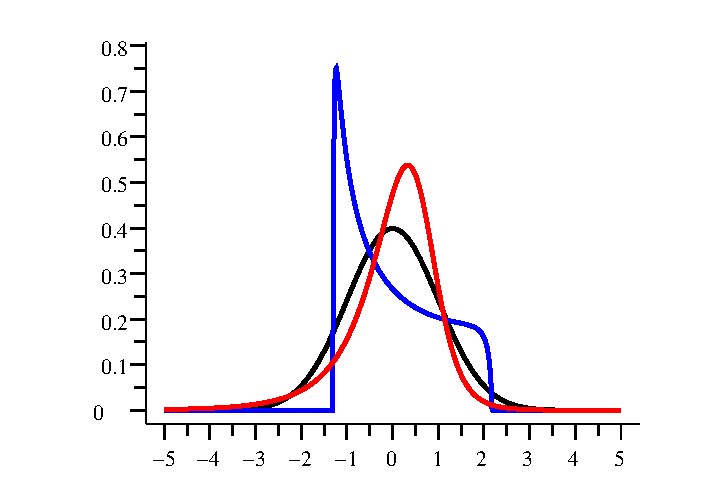
\includegraphics[width=0.6\textwidth]{johnson_examples.pdf}
\caption{ Black: $s = 0,  ~k = 3$, Gaussian. Red: $s = -1.5, ~k = 10$, $S_{U}$.
Blue: $s = 0.5, ~ k = 2$, $S_{B}$.
For all three curves, the mean is 0 and the standard deviation is 1.}
\label{johns_exa}
\end{center}
\end{figure}

Johnson's $S_{U}$ and $S_{B}$ curves are implemented in NPStat with classes
\cname{JohnsonSu} and \cname{JohnsonSb}, respectively (header file
``npstat/stat/JohnsonCurves.hh''). Both of these
distributions are parameterized by $\mu$, $\sigma$, $s$, and $k$,
with an automatic internal conversion into $\xi, \lambda, \gamma, \delta$.
An original algorithm was developed to perform this conversion,
based in part on ideas from Refs.~\cite{ref:draper, ref:hill}.
The lognormal distribution parameterized by $\mu$, $\sigma$, and $s$
is implemented by the \cname{LogNormal} class (header file
``npstat/stat/Distributions1D.hh''). The class \cname{JohnsonSystem}
(header file ``npstat/stat/JohnsonCurves.hh'') can be used when automatic
switching between $S_{U}$, $S_{B}$,
lognormal, and Gaussian distributions is desired.


\subsection{Composite Distributions}

Composite distributions are built out of two or more
component distributions. One of these component distributions is
arbitrary while
all others must have a density supported on the interval
[0, 1]. Suppose, $G_k(x), \ k = 1, 2, 3, ...$ are cumulative
distribution functions with corresponding densities $g_i(x)$
proportional to $I(0 \le x \le 1)$.
Then, if $H(x)$ is a cumulative distribution function
with density $h(x)$, $F_1(x) = G_1(H(x))$ is also a cumulative
distribution function with density $f_1(x) = h(x) \, g_1(H(x))$.
Similarly, $F_2(x) = G_2(F_1(x))$ is a cumulative distribution with density
$f_2(x) = f_1(x) g_2(F_1(x)) = h(x) \, g_1(H(x)) g_2(G_1(H(x)))$.
We can now construct $F_3(x) = G_3(F_2(x))$ and so on. This sequence can
be terminated after an arbitrary number of steps.

Note that $f_1(x) = h(x)$ in case $g_1(x)$ is a uniform
probability density. Small deviations from uniformity in $g_1(x)$
will lead to corresponding small changes in $f_1(x)$.
The resulting density model can be quite flexible, even if
the component distributions $H(x)$ and $G_1(x)$ are
simple. Therefore, data samples with complicated sets
of features can be modeled as follows: construct
an approximate model $h(x)$ first, even if it does not fit
the sample quite right.
Then transform the data points $x_i$ to the [0, 1] interval
according to $y_i = H(x_i)$. The density of 
points $y_i$\footnote{This density is called ``relative density'' 
in the statistical literature~\cite{ref:handcock}. Note
that $h(x)$ should be selected in such a way that the ratio between
the unknown population density of the sample under study and $h(x)$ should
be bounded for all $x$. If it is not, the relative density
will usually be unbounded, and its subsequent representation
by polynomials or log-polynomials will not lead to a consistent
estimate. Johnson curves often work reasonably well as $h(x)$.}
can now be
fitted to another parametric distribution (including composite one)
or it can be modeled by nonparametric techniques~\cite{ref:kdetransform}.
Due to the elimination of the boundary bias, the LOrPE density
estimation method described in Section~\ref{sec:lorpe}
becomes especially useful in the latter approach.
Once the appropriate $G(y)$ is constructed (parametrically
or not), the resulting composite density will provide
a good fit to the original set of points $x_i$\footnote{There is,
of course, a close connection between this density modeling
approach and a number of goodness-of-fit techniques based on
the comparison of the empirical cdf
with the cdf of the fitted density. For example, using
Legendre polynomials to model $\log (g_1(x))$, as in the
\cname{LogQuadratic1D} density, directly
improves the test criterion used in the Neyman's
smooth test for goodness-of-fit~\cite{ref:thas, ref:smoothtest}.}.

The composite distributions are implemented in NPStat
with the \cname{CompositeDistribution1D} class.
One composite distribution can be used to construct
another, thus allowing for composition chains of
arbitrary length, as described at the beginning of
this subsection. Several pre-built distributions of this type
are included in the NPStat package (they are declared in the header file
``npstat/stat/CompositeDistros1D.hh''). Flexible
models potentially capable of fitting wide varieties
of univariate data samples are implemented by the \cname{JohnsonLadder}
and \cname{BinnedCompositeJohnson} classes. In both of these,
Johnson curves are used as $H(x)$. \cname{JohnsonLadder}
takes an arbitrarily long sequence of parametric \cname{LogQuadratic1D}
distributions for $G_k(x)$ while \cname{BinnedCompositeJohnson}
is using a single nonparametric \cname{BinnedDensity1D} as $G_1(x)$.


\subsection{Univariate Discrete Distributions}

Classes which represent univariate discrete distributions
inherit from the \cname{AbsDiscreteDistribution1D} abstract base class.
The interface defined by this base class differs in a number of ways
from the \cname{AbsDistribution1D} interface.
Instead of the method \cname{density}
used with arguments of type ``double'',
discrete distributions have the method \cname{probability} defined for
the arguments of type ``long int''.
The methods \cname{cdf} and \cname{exceedance}
have the same signatures as corresponding methods of continuous distributions,
but the \cname{quantile} function is returning long integers. The
method \cname{random} generates long integers as well.

Discrete univariate distributions which can be trivially shifted should
inherit from the \cname{ShiftableDiscreteDistribution1D} base class which
handles the shift operation. There is, however, no operation analogous
to scaling of continuous distributions.

Univariate discrete distributions implemented
in NPStat are listed in Table~\ref{table:discrdistros1d}.
\begin{table}[ht!]
\caption{Discrete univariate distributions included in NPStat.
The location parameter is not shown explicitly for shiftable distributions.
Classes listed in this table are declared in the header file
``npstat/stat/DiscreteDistributions1D.hh''.}
\label{table:discrdistros1d}
\begin{center}
\noindent\begin{tabular}{|c|c|c|} \hline
Class Name & $p(n)$ & Shiftable? \\ \hline\hline
\cname{DiscreteTabulated1D} & \begin{minipage}{0.52\linewidth}
                      \vskip1mm
                      Defined by a table of probability values.
                      Normalization is computed automatically.
                      \end{minipage} & yes \\ \hline
\cname{Poisson1D} & $\frac{\lambda^n}{n!} e^{-\lambda}$ & no \\ \hline
\end{tabular}
\end{center}
\end{table}
Mixtures of discrete univariate distributions with finite support
can be implemented using the function \cname{pooledDiscreteTabulated1D}
(header file ``npstat/stat/DiscreteDistributions1D.hh'').

\subsection{Multivariate Continuous Distributions}

All classes which represent multivariate continuous distributions
inherit from the \cname{AbsDistributionND} abstract base class.
These classes must implement methods \cname{density} (probability
density function) and \cname{unitMap} (mapping from the unit
$d$-dimensional cube, $U_d$, into the density support region).
Densities that can be shifted and scaled in each coordinate separately
should be derived from the \cname{AbsScalableDistributionND} base class
(which itself inherits from \cname{AbsDistributionND}).
Classes representing densities that look like $p({\bf x}) = \prod q(x_i)$,
where $q(x)$ is some one-dimensional density,
should be derived from the \cname{HomogeneousProductDistroND} base class
(the three base classes just mentioned
are declared in the ``npstat/stat/AbsDistributionND.hh'' header file).
Simple classes inheriting from \cname{AbsDistributionND}
are listed in Table~\ref{table:distrosnd}.
\begin{table}[ht!]
\caption{Continuous multivariate distributions included in NPStat.
These distributions are predominantly intended for use as multivariate
density estimation kernels.
Shifts and scale factors are not shown for scalable distributions.
Here, ``scalability'' means
the ability to adjust the shift and scale parameters in each
dimension, not the complete bandwidth matrix.
When not given explicitly, the normalization constant $\cal{N}$
ensures that 
$\int p({\bf x}) d{\bf x} = 1$. All of these distributions
are declared in the header file ``npstat/stat/DistributionsND.hh''
with exception of \cname{ScalableGaussND} which has its own header.}
\label{table:distrosnd}
\begin{center}
\noindent\begin{tabular}{|c|c|c|} \hline
Class Name & $p({\bf x})$ & Scalable? \\ \hline\hline
\cname{ProductDistributionND} &  $\prod_{i=1}^{d} p_i(x_i)$ & 
\begin{minipage}{0.13\linewidth}
depends on components
\end{minipage} \\ \hline
\cname{UniformND} & $\prod_{i=1}^{d} I(0 \le x_i \le 1)$ & yes \\ \hline
\cname{ScalableGaussND} & $(2 \pi)^{-d/2} e^{-|{\bf x}|^2/2}$ & yes \\ \hline
\cname{ProductSymmetricBetaND} & ${\cal{N}} \prod_{i=1}^{d} (1 - x_i^2)^p I(-1 < x_i < 1)$ & yes \\ \hline
\cname{ScalableSymmetricBetaND} & ${\cal{N}} (1 - |{\bf x}|^2)^p I(|{\bf x}| < 1)$ & yes \\ \hline
\cname{ScalableHuberND} & ${\cal{N}} \, [e^{-|{\bf x}|^2/2} I(|{\bf x}| \le a) + e^{\, a (a/2 - |{\bf x}|)} (1 - I(|{\bf x}| \le a))]$ & yes \\ \hline
\cname{RadialProfileND} & \begin{minipage}{0.52\linewidth}
                      \vskip1mm
                      Arbitrary centrally-symmetric density.
                      Defined by its radial profile:
                      a table of equidistant values on
                      the [0, 1] interval, interpolated by 
                      a~polynomial (up to cubic). The first table
                      point is at $|{\bf x}| = 0$ and the last is at
                      $|{\bf x}| = 1$. For $|{\bf x}| > 1$ the density is 0.
                      Normalization is computed automatically.
                      \end{minipage} & yes \\ \hline
\cname{BinnedDensityND} & \begin{minipage}{0.52\linewidth}
                      \vskip1mm
                      Defined by a table of values
                      on $U_d$, equidistant in each dimension,
                      with optional multilinear
                      interpolation. In each dimension,
                      the first table point is at
                      $x_i = 1/(2 N_i)$ and the last is at
                      $x_i = 1 - 1/(2 N_i)$.
                      Useful for converting multivariate
                      histograms into distributions.
                      \end{minipage} 
& yes \\ \hline
\end{tabular}
\end{center}
\end{table}


\subsection{Copulas}

For any continuous multivariate density $p({\bf x}|{\bf a})$ 
in a $d$-dimensional space $X$ of random variables ${\bf x} \in X$
depending on a vector of parameters ${\bf a}$,
we define $d$ marginal densities $p_i(x_i|{\bf a})$, $i = 1, \ldots, d$ by
$$
p_i(x_i|{\bf a}) \equiv \int p(x_1, \ldots, x_d |{\bf a}) \mathop{\prod_{j=1}^d}_{j \ne i} d x_j
$$
with their corresponding cumulative distribution functions
$$
F_i(x_i|{\bf a}) \equiv \int_{-\infty}^{x_i} p_i(\tau|{\bf a}) d \tau .
$$
For each point ${\bf x} \in X$, there is a corresponding
point ${\bf y}$ in a unit $d$-dimensional
cube $U_d$ such that $y_i(x_i) \equiv F_i(x_i|{\bf a})$, $i = 1, \ldots, d$. The {\it copula density}
is defined on $U_d$ by
\begin{equation}
c({\bf y}({\bf x})|{\bf a}) \equiv \frac{p({\bf x}|{\bf a})}{\prod_{i=1}^{d} p_i(x_i|{\bf a})}.
\label{eq:copuladef}
\end{equation}
Copula density (as well as its corresponding multivariate
distribution function $C({\bf y}|{\bf a})$, or just {\it copula})
contains all information
about mutual dependence of individual variables $x_i$.
It can be shown that all copula marginals are uniform and, conversely,
that any distribution on $U_d$ whose marginals are uniform
is a copula~\cite{ref:copulabook}.

Naturally, when the copula and the marginals of some multivariate density
are known, the density itself is expressed by
\begin{equation}
p({\bf x}|{\bf a}) = c({\bf y}({\bf x})|{\bf a}) \prod_{i=1}^{d} p_i(x_i|{\bf a}).
\end{equation}
Note that $c({\bf y}|{\bf a}) = 1$ for all ${\bf y}$ if and only if all $x_i$
are independent and the density $p({\bf x}|{\bf a})$ is fully
factorizable.

The NPStat package allows its users to model multivariate continuous
distributions using copula and marginals with the aid of
\cname{CompositeDistributionND} class. An object of this class is
normally constructed out of user-provided copula and marginals.
\cname{CompositeDistributionND} object can also be constructed
from histogram bins. Several standard copulas are
implemented: Gaussian, Student's-$t$, and
Farlie-Gumbel-Morgenstern~\cite{ref:copulabook}.
The corresponding class names are \cname{GaussianCopula},
\cname{TCopula}, and \cname{FGMCopula} (these classes are
declared in the header file ``npstat/stat/Copulas.hh'').

Empirical multivariate copulas densities can be constructed
as follows. Let's assume that there are no coincident 
point coordinates in each dataset variable. We can sort all
$N$ elements of the data set in the increasing order in each coordinate
separately and assign to each data point $i$ a multi-index
$\{m_{i0}, ..., m_{id}\}$. For each dimension $k$, $m_{ik}$
represents the number of the point $i$ in the sequence ordered
by the dimension $k$ coordinate, so that
$0 \le m_{ik} < N$. The empirical copula density, $\mbox{ECD}({\bf x})$,
is then defined by
\begin{equation}
\mbox{ECD}({\bf x}) = \sum_{i=0}^{N-1} \prod_{k=0}^{d-1} \delta\left(x_k - \frac{m_{ik} + 1/2}{N}\right),
\end{equation}
where $\delta(x)$ is the Dirac delta function. To get a better idea about
locations of these delta functions, think of
an $N \times N \times ... \times N$ uniform grid in $d$ dimensions on
which $N$ points are placed in such a way that no two
points share the same coordinate in any of the dimensions.
In two dimensions, this is like the placement of chess pieces
in the eight queens puzzle~\cite{ref:eightqueens}
which is simplified to use rooks instead of queens~\cite{ref:eightrooks}.

In the NPStat package, empirical copula densities can be approximated by
histograms defined on $U_d$. Construction of empirical copula histograms
can be performed by functions \cname{empiricalCopulaHisto} 
(header file ``npstat/stat/empiricalCopulaHisto.hh'') and
\cname{empiricalCopulaDensity} 
(header file ``npstat/stat/empiricalCopula.hh''). The integrated empirical copulas can be
constructed on uniform grids by the \cname{calculateEmpiricalCopula}
function (header ``npstat/stat/empiricalCopula.hh''). 

The Spearman's rank correlation coefficient, $\rho$, can
be estimated from two-dimensional empirical copulas using functions
\cname{spearmansRhoFromCopula} and \cname{spearmansRhoFromCopulaDensity}
declared in the header file ``npstat/stat/spearmansRho.hh''.
These functions evaluate the following integrals numerically:
\begin{align}
  \rho &= 12 \int_0^1 \int_0^1 C({\bf y}|{\bf a}) dy_0 dy_1 - 3 & \mbox{\ } & \mbox{used by \textsf{spearmansRhoFromCopula}} \\
  \rho &= 12 \int_0^1 \int_0^1 c({\bf y}|{\bf a}) y_0 y_1 dy_0 dy_1 - 3 & \mbox{\ } & \mbox{used by \textsf{spearmansRhoFromCopulaDensity}}
\end{align}
While these two formulas are identical mathematically~\cite{ref:copulabook},
the approximations used
in numerical integration and differentiation will usually lead to slightly
different results returned by these functions for some copula and its
corresponding density.

The Kendall's rank correlation coefficient, $\tau$,
can be estimated from the empirical copulas using the
function \cname{kendallsTauFromCopula} declared in
the header ``npstat/stat/kendallsTau.hh''.
This function evaluates the following formula numerically:
\begin{equation}
\tau = 4 \int_0^1 \int_0^1  C({\bf y}|{\bf a}) c({\bf y}|{\bf a}) dy_0 dy_1 - 1.
\end{equation}

The mutual information between variables can be estimated from
copula densities represented on uniform grids according
to Eq.~\ref{eq:entropy}\footnote{Mutual information is
simply the negative of the copula entropy~\cite{ref:copulaentropy}.}.

Decomposition of multivariate densities into the marginals and the
copula is useful not only for a subsequent analysis of mutual
dependencies of the variates but also for implementing nonparametric
density interpolation, as described in the next section.


\section{Nonparametric Interpolation of Densities}
\label{sec:densityinterpolation}

There are numerous problems in High Energy Physics in which construction of some
probability density requires extensive simulations and, due to the CPU
time limitations, can only be performed for a~limited number of
parameter settings. This is typical, for example, for ``mass
templates'' which depend on such parameters as the pole mass of the
particle under study, sample background fraction, detector jet energy
scale, {\it etc}. It is often desirable to have the capability to
evaluate such a density for arbitrary parameter values. 
It is sometimes possible to address this problem by postulating
an explicit parametric
model and fitting that model to the sets of simulated distributions.
However, complex dependence of the distribution shapes on the parameter
values often leads to infeasibility of this approach. Then it becomes
necessary to interpolate the densities without postulating a concrete
model.

\subsection{Interpolation of Univariate Densities using Quantile Functions}
\label{sec:interpolatebyquant}

As it was shown in~\cite{ref:read}, a general
interpolation of one-dimensional distributions which
leads to very naturally looking results
can be achieved by
interpolating the {\it quantile function} (defined as the
inverse of the cumulative distribution function). While study~\cite{ref:read}
considers linear interpolation in one-dimensional parameter space, it is obvious that
similar weighted average interpolation can be easily constructed in
multivariate parameter settings and with higher order interpolation
schemes. In general, the interpolated quantile function for  
an~arbitrary parameter value ${\bf a}$ is expressed by
\begin{equation}
\label{eq:quantileinterp1d}
q(y|{\bf a}) =  \sum_{j=1}^m w_j q(y|{\bf a}_j),
\end{equation}
where the weighted quantile functions are summed at the $m$ ``nearby''
parameter settings ${\bf a}_j$ for which the distribution was
explicitly constructed. The weights $w_j$ are normalized by
$\sum_{j=1}^m w_j = 1$.  Their precise values depend on the location
of ${\bf a}$ w.r.t. nearby ${\bf a}_j$ and on the interpolation scheme used.
Simple high-order interpolation schemes can be constructed
in one-dimensional parameter space by using Lagrange interpolating
polynomials
to determine the weights\footnote{To determine interpolated value of a function using
Lagrange interpolating polynomials, weights are assigned to function
values at a set of nearby points according to a rule
published by Lagrange in 1795. The weights depend only on the
abscissae of the interpolated points and on the coordinate
at which the function value is evaluated but not on the
interpolated function values.}. In $r$-dimensional parameter
space, rectangular grids can be utilized with multilinear or
multicubic interpolation. For
example, in the case of multilinear
interpolation, the weights can be calculated as follows:
\begin{thinlist}
\item Find the hyperrectangular parameter grid
cell inside which the value of ${\bf a}$ falls.
\item Shift and scale this cell so that it becomes a hypercube
with diagonal vertices at $(0, 0, ..., 0)$ and $(1, 1, ..., 1)$.
\item Let's designate the shifted and scaled value of ${\bf a}$ by ${\bf z}$,
      with components $(z_1, z_2, ..., z_r)$.
      If we were to interpolate towards ${\bf z}$ 
      a scalar function $f$ defined at the
      vertices with coordinates $(c_1, c_2, \ldots, c_r)$,
      where all $c_k$ values are now either 0 or 1,
      then we would use the formula
      \begin{equation}
      \label{eq:multilinear}
f(z_1, z_2, ..., z_r) = \sum_{\substack{
c_1 \in \,\{0, 1\}\\
c_2 \in \,\{0, 1\}\\
\cdot \cdot \cdot \cdot \cdot \cdot \cdot \cdot \cdot \\
c_r \in \,\{0, 1\}\\
}}  f(c_1, c_2, ..., c_r) \prod_{k=1}^r z_k^{c_k} (1 - z_k)^{1 - c_k}
      \end{equation}
      which is obviously linear in every $z_k$ and has
      correct function values when evaluated at the vertices.
      In complete analogy, we define the weights for the quantile functions
      constructed at the vertices with coordinates $(c_1, c_2, \ldots, c_r)$ to be
      $w(c_1, c_2, \ldots, c_r) = \prod_{k=1}^r z_k^{c_k} (1 - z_k)^{1 - c_k}$.
      Naturally, there are $m = 2^r$ weights total.
\end{thinlist}
The quantile interpolation of univariate distributions is implemented
in the NPStat package with the \cname{InterpolatedDistribution1D} class.
A collection of quantile functions is assembled incrementally together
with their weights (formula for calculating the weights is to be supplied
by the user).
For calculating the interpolated density at point $x$,
the equation $x = q(y|{\bf a})$,
with $q(y|{\bf a})$ from~\ref{eq:quantileinterp1d},
is solved numerically for $y$. The density is then evaluated by
numerically differentiating the interpolated quantile function:
$p(x|{\bf a}) = \left( \frac{\partial q(y|{\bf a})}{\partial y} \right)^{-1}$.

A class with a simpler interface implementing linear weight assignments
between nearby points in a 1-d parameter space is called \cname{InterpolatedDistro1D1P}.

Less reliable but computationally faster linear interpolation of densities (instead of
quantile functions) is implemented for 1-d parameter spaces by the
class \cname{VerticallyInterpolatedDistro1D1P}. This class allows
the user to perform interpolation in a transformed space (for example,
the transform can center all distributions at 0 and rescale them to
the same width) in order to alleviate deficiencies of ``vertical''
interpolation.


\subsection{Interpolation of Multivariate Densities}
\label{sec:interpolatemultivar}

The procedure described in the previous section can be
generalized to interpolate multivariate distributions.
Let $p({\bf x}|{\bf a})$ be a multivariate probability density
in a $d$-dimensional space $X$ of random variables ${\bf x} \in X$.
${\bf a}$ is a vector of parameters, and
$\int_{X} p({\bf x}|{\bf a}) d {\bf x} = 1$ 
for every ${\bf a}$\footnote{Compared to interpolation of
arbitrary functions, preserving this normalization is one of the
major complications in interpolating multivariate densities.}.
For a~``well-behaved'' density (Riemann-integrable, {\it etc}),
it is always possible to construct a one-to-one
mapping from the space $X$
into the unit $d$-dimensional cube, $U_d$, using a sequence of one-dimensional
conditional cumulative distribution functions. These functions are defined
as follows:
$$
\begin{array}{c}
F_{1}(x_1|x_2, x_3, \ldots, x_d, {\bf a}) \equiv \int_{-\infty}^{x_1} p(z_1, x_2, x_3, \ldots, x_d | {\bf a}) d z_1 / 
\int_{-\infty}^{\infty} p(z_1, x_2, x_3, \ldots, x_d | {\bf a}) d z_1
\\
F_{2}(x_2 | x_3, \ldots, x_d, {\bf a}) \equiv \int_{-\infty}^{x_2} F_{1}(\infty | z_2, x_3, \ldots, x_d, {\bf a}) d z_2 /
\int_{-\infty}^{\infty} F_{1}(\infty | z_2, x_3, \ldots, x_d, {\bf a}) d z_2
\\
F_{3}(x_3 | \ldots, x_d, {\bf a}) \equiv \int_{-\infty}^{x_3} F_{2}(\infty | z_3, \ldots, x_d, {\bf a}) d z_3 /
\int_{-\infty}^{\infty} F_{2}(\infty | z_3, \ldots, x_d, {\bf a}) d z_3
\\
.\ .\ .\ .\ .\ .\ .\ .\ .\ .\ .\ .\ .\ .\ .\ .\ .\ .\ .\ .\ .\ .\ .\ .\ .\ .\ .\ .\ .\ .\ .\ .\ .\ .\ .\ .\ .\ .\ .\ .\ .\ .\ .\ .\ .\ .\ .
\\
F_{d}(x_d | {\bf a}) \equiv \int_{-\infty}^{x_d} F_{d-1}(\infty | z_d, {\bf a}) d z_d /
\int_{-\infty}^{\infty} F_{d-1}(\infty | z_d, {\bf a}) d z_d
\end{array}
$$
Naturally, $F_{k}(\infty | x_{k+1}, \ldots, x_d, {\bf a})$ is just renormalized $p({\bf x}|{\bf a})$
in which the first $k$ components of ${\bf x}$ are integrated out ({\it i.e.,} marginalized).
The mapping from ${\bf x} \in X$ into ${\bf y} \in U_d$ is defined by $y_i = F_i(x_i | \ldots), \ i = 1, \ldots, d$. In terms of conditional cumulative distribution functions,
$$
p({\bf x}|{\bf a}) = \prod_{i=1}^{d}{\frac{\partial F_i(x_i | \ldots)}{\partial x_i}}.
$$

This method is not unique and other mappings 
from $X$ to $U_d$ are possible. What makes this particular construction useful
is that the inverse mapping, from $U_d$ into $X$, can be
easily constructed as well: we simply solve the equations 
\begin{equation}
\label{eq:invertcondcdf}
y_i = F_i(x_i | \ldots)
\end{equation}
in the reverse order, starting from dimension $d$ and going back
to dimension $1$. Each equation in this sequence {\it has only one unknown}
and therefore it can be efficiently solved numerically
(and sometimes algebraically) by a variety
of standard root finding techniques. The solutions of these equations,
$x_i = q_i(y_i | x_{i+1}, \ldots, x_d, {\bf a}) \equiv F_i^{-1}(y_i | \ldots)$, are
the {\it conditional quantile functions} (CQFs). Note that
\begin{equation}
\label{eq:invderiv}
p({\bf x}|{\bf a}) = \left( \prod_{\ i=1}^{d}{\frac{\partial q_i(y_i | \ldots)}{\partial y_i}} \right)^{-1}.
\end{equation}

Now, if the CQFs are known for some parameter values
${\bf a}_1$ and ${\bf a}_2$,
interpolation towards ${\bf a} = (1 - \lambda) {\bf a}_1 + \lambda {\bf a}_2$ is made
in the same manner as described in Section~\ref{sec:interpolatebyquant}: 
$x_i = (1 - \lambda) q_i(y_i | x_{i+1}, \ldots, x_d, {\bf a}_1) + \lambda q_i(y_i | x_{i+1}, \ldots, x_d, {\bf a}_2)$.
If the CQFs 
are known on a~grid in the parameter space, we have to use
an appropriate interpolation technique (multilinear, multicubic, {\it etc})
in that space in order to assign
the weights to the CQFs at the nearby grid points. In general,
the interpolated CQFs are defined by
a weighted average
\begin{equation}
\label{eq:interpq}
q_i(y_i | x_{i+1}, \ldots, x_d, {\bf a}) = \sum_{j=1}^m w_j q_i(y_i | x_{i+1}, \ldots, x_d, {\bf a}_j),
\end{equation}
where the sum is performed over $m$ nearby parameter points,
weights $w_j$ are normalized by $\sum_{j=1}^m w_j = 1$, and their
exact values depend on the parameter grid chosen and the interpolation method
used.

Basically, it is the whole mapping from ${\bf y}$ into ${\bf x}$ which gets
interpolated in this method.
The CQF interpolation results look 
very natural, but the process is rather CPU-intensive:
for each ${\bf x}$ we need to solve $d$ one-dimensional nonlinear equations
\begin{equation}
\label{eq:interpsolve}
x_i = q_i(y_i | x_{i+1}, \ldots, x_d, {\bf a}), \ \ \ \ i = d, \ldots, 1
\end{equation}
in order to determine ${\bf y}$ of the interpolated mapping.
In this process, each call to evaluate $q_i(y_i | x_{i+1}, \ldots, x_d, {\bf a})$
triggers $m$ calls to evaluate $q_i(y_i | x_{i+1}, \ldots, x_d, {\bf a}_j)$.
Depending on implementation details, each of these $m$ calls
may in turn trigger root finding in an equation
like~\ref{eq:invertcondcdf}.
Once ${\bf y}$ is found for the interpolated CQFs,
density is determined by numerical
evaluation of~\ref{eq:invderiv}
in which $q_i(y_i | \ldots)$ are given by~\ref{eq:interpq}.

In practice, finite steps of the parameter grids will cause
dependence of the interpolation results on the order in which
conditional quantiles are evaluated. If choosing some
particular order is considered undesirable and increased CPU
loads are acceptable, all $d!$ possible permutations
should be averaged.

In the NPStat package, multivariate densities whose mapping
from the multidimensional unit cube into the density support
region is implemented via CQFs return ``true'' when
their virtual function \cname{mappedByQuantiles} is called.
User-developed implementations of
multivariate densities should follow this convention as well.
In particular, mapping of
the densities represented by the \cname{BinnedDensityND} class
(lookup tables on hyperrectangular
grids with multilinear interpolation) is performed by CQFs,
as well as mapping of all fully factorizable densities. 

When the fidelity of the model is less critical or when the
correlation structure of the distribution is more stable w.r.t.
parameter changes than its location and scales, much faster
multivariate density interpolation can be performed by decomposing
the density into the copula and the marginals. The support
of the copula density $c({\bf y}({\bf x})|{\bf a})$ defined
in Eq.~\ref{eq:copuladef}
is always $U_d$ and it does not depend on the
parameter ${\bf a}$. This suggests that the marginals and the copula can
be interpolated separately, using quantile function interpolation
for the marginals and the standard weighted average interpolation
for the copula.

The NPStat package uses the same data structure to perform both
CQF-based and copula-based interpolation of multivariate densities.
Multilinear interpolation is supported on a rectangular parameter
grid (not necessarily equidistant).
The distributions at the grid points are collected together
using the \cname{GridInterpolatedDistribution} template,
while method-specific
differences are isolated inside a policy class which serves as
the \cname{GridInterpolatedDistribution} template parameter.
Currently, \cname{UnitMapInterpolationND} or 
\cname{CopulaInterpolationND} classes can serve as such a~parameter
which results in CQF-based or copula-based interpolation, respectively.

\section{Nonparametric Density Estimation}
\label{sec:densityestimation}

The problem of estimating population probability density function
from a finite sample drawn from this population is ubiquitous
in data analysis practice. It is often the case that
there are no substantial reasons for choosing a particular parametric
density model but certain assumptions,
such as continuity
of the density together with some number of derivatives or absence
of narrow spatial features, can still be justified. There is
a~number of approaches by which assumptions of this kind can be introduced
into the statistical model. These approaches are collectively known
as ``nonparametric
density estimation'' methods~{\cite{ref:silverman, ref:izenmann, ref:kde}}. The NPStat
package provides an efficient implementation of one of 
such methods, kernel density estimation (KDE), together with its extension
to polynomial density models and densities with bounded support. 
This extension is called ``local orthogonal polynomial expansion'' (LOrPE).

\subsection{Kernel Density Estimation (KDE)}
\label{sec:kde}

Suppose, we have an i.i.d.~sample of measurements $x_i$, $i = 0, 1,
..., N-1$ from a univariate probability density $p(x)$. The empirical
probability density function (EPDF) for this sample is defined by
\begin{equation}
\mbox{EPDF}(x) = \frac{1}{N} \sum_{i=0}^{N-1} \delta (x - x_i),
\label{eq:edf}
\end{equation}
where $\delta(x)$ is the Dirac delta function. $\mbox{EPDF}(x)$
can itself be considered an estimate of $p(x)$. However, this
estimate can be substantially improved if some additional information
about $p(x)$ is available. For example, we can often assume that
$p(x)$ is continuous together with its first few derivatives or
that it can have at most a few modes. In such cases a convolution
of $\mbox{EPDF}(x)$ with a kernel function, $K(x)$, often provides
a much better estimate of the population density. $K(x)$ itself is
usually chosen to be a symmetric continuous density with a location
and scale parameter, so that the resulting estimate looks
like
\begin{equation}
\hat{p}\sub{KDE}(x|h) = \frac{1}{N h} \sum_{i=0}^{N-1} K \left(\frac{x - x_i}{h}\right).
\label{eq:kde}
\end{equation}
 In the context of
density estimation, parameter $h$ is usually referred to as
``bandwidth''.
Use of the Gaussian distribution or one of the distributions from the
symmetric beta family as $K(x)$ is very common. In fact, it is so common
that beta family kernels have their own names in the density estimation
literature. These names are listed in Table~\ref{table:betakernels}.
\begin{table}[h!]
\caption{One-dimensional kernels from the symmetric beta family.
All these kernels look like
${\cal{N}} \, (1 - x^2)^p \, I(-1 < x < 1)$, where ${\cal{N}}$
is the appropriate normalization factor. In the
NPStat package, their formulae are implemented by the
\cname{SymmetricBeta1D} function.}
\label{table:betakernels}
\begin{center}
\noindent\begin{tabular}{|c|c|} \hline
Kernel name  & Power $p$ \\ \hline\hline
Uniform (also called ``boxcar'') & 0 \\ \hline
Epanechnikov & 1 \\ \hline
Biweight (also called ``quartic'') & 2 \\ \hline
Triweight & 3 \\ \hline
Quadweight & 4 \\ \hline
% Quintweight & 5 \\ \hline
\end{tabular}
\end{center}
\end{table}

In the limit $N \rightarrow \infty$ and with proper choice of $h$ so that
$h \rightarrow 0$ and $N h \rightarrow \infty$,
$\hat{p}\sub{KDE}(x)$ becomes a~consistent
estimate of $p(x)$ in terms of integrated squared error (ISE):
\begin{equation}
\mbox{ISE}(h) = \int_{-\infty}^{\infty} (\hat{p}\sub{KDE}(x|h) - p(x))^2 dx, \ \ \ \ \ \lim_{N \rightarrow \infty} \mbox{ISE}(h) = 0.
\end{equation}

For the method analysis purposes, it is useful to understand
what happens when we reconstruct known densities $p(x)$.
Here, another measure of distance between the true
density and its estimator becomes indispensable,
called ``mean integrated squared error'' (MISE):
\begin{equation}
\mbox{MISE}(h) = E(\mbox{ISE}(h)) = E \left( \int_{-\infty}^{\infty} (\hat{p}\sub{KDE}(x|h) - p(x))^2 dx \right),
\label{eq:mise}
\end{equation}
where $E(...)$ stands for the expectation value over samples of $N$ points
drawn from $p(x)$. 
While other distance measures can be defined
(and may be more relevant for your problem),
$\mbox{MISE}(h)$ is usually
the easiest to analyze
mathematically\footnote{Note that both ISE and MISE are not dimensionless and,
therefore, not invariant under scaling transformations.
It is OK to compare different $\hat{p}\sub{KDE}(x|h)$ with each other if
the underlying $p(x)$ is the same, but ISE or MISE comparison for different $p(x)$
requires certain care if meaningful results are to be obtained.}.
A typical goal of such an analysis consists in
finding the value of $h$ which minimizes $\mbox{MISE}(h)$ for
a~sample of given size, and a~significant amount of effort
has been devoted to such bandwidth optimization studies
(see, {\it e.g.,} Refs.~\cite{ref:bwopt, ref:loaderbw} for a review).
A large fraction of these studies employs a~simple MISE approximation valid for large
values of $N$ known as ``AMISE'' (asymptotic MISE). This approximation
includes just the two leading terms known as ``bias'' which increases with
increasing bandwidth and ``variance'' which decreases with increasing bandwidth,
so that the bandwidth optimization procedure is reduced to finding
the best bias-variance trade-off.

For subsequent discussion, it will be useful to introduce the concept
of kernel order. Let's define the functional
\begin{equation}
\mu_{j}(f) = \int_{-\infty}^{\infty} x^j f(x) dx
\label{eq:mufunct}
\end{equation}
which is the $j$-th moment of $f(x)$ about 0.
Then it is said that the kernel $K(x)$ is of order $m$ if
\begin{equation}
\mu_0(K) = 1, \ \mu_j(K) = 0 \ \mbox{for} \ j = 1, ..., m-1, \ \mbox{and} \ \mu_m(K) \ne 0.
\end{equation}
It can be shown that, for one-dimensional
KDE, the rate of AMISE convergence to 0 is proportional
to $N^{-\frac{2 m}{2 m + 1}}$ (see, for example, section~2.8
of~\cite{ref:kernsmooth}). Therefore, kernels with high values
of $m$ should be preferred for large samples. At the same time,
only in case $m = 2$ the kernels can be everywhere non-negative
({\it i.e.,} bona fide densities).
When $m > 2$ (so called ``high-order'' kernels), in order to have
$\mu_2(K) = 0$, $K(x)$ must become negative somewhere.
Therefore, negative values of $\hat{p}\sub{KDE}(x|h)$ also
become possible, and a mechanism for dealing with this problem
must be specified. In NPStat, this problem is normally taken care
of by setting negative values of $\hat{p}\sub{KDE}(x|h)$ to 0
with subsequent renormalization of the density estimate so that its
integral is 1.

It is instructive to consider $p(x)$, $\mbox{EPDF}(x)$,
and $\hat{p}\sub{KDE}(x|h)$ in the frequency
domain\footnote{The Fourier transform of a
probability density is called ``characteristic function'' of the distribution.}. There, the Fourier
transform of $K(x)$ acts as a low-pass filter which suppresses the sampling
noise present in $\mbox{EPDF}(x)$ so that the result, $\hat{p}\sub{KDE}(x|h)$,
has a better match
to the spectrum of $p(x)$. By Parseval's identity, this
leads to the reduction of the ISE. High-order kernels allow
for a sharper frequency cutoff in the filter. Fortunately, the precise shape
of $p(x)$ frequency spectrum
is relatively
unimportant, it is only important that its high frequency components
decay ``fast enough'' so that their suppression together with the
noise does not cause a significant distortion of  $\hat{p}\sub{KDE}(x|h)$
in comparison with $p(x)$. Powerful automatic bandwidth selection rules
can be derived from this type of analysis if certain
assumptions about the $p(x)$ spectrum decay rate
at high frequencies are satisfied~\cite{ref:chiu2, ref:chiumultivar}.

With a few modifications, the ideas described above can be translated
to multivariate settings. The kernel function becomes a multivariate
density, and the bandwidth parameter becomes, in general, the bandwidth
matrix (for example, the covariance matrix in the case of multivariate
Gaussian kernel).

The NPStat package calculates $\hat{p}\sub{KDE}(x|h)$ on an equidistant
grid in one or more dimensions.
Initially, the data sample is histogrammed using a finely
binned histogram and then convoluted with a kernel using
Discrete Fast Fourier Transform (DFFT).
The number of histogram bins, $N_b$, should be selected
taking into account the following considerations:
\begin{thinlist}
\item The bins should be sufficiently small so that no ``interesting''
      detail will be missed due to discretization of the density.

\item The bins should be sufficiently small so that the expected optimal
      MISE is significantly larger than the ISE due to
      density discretization. Detailed exposition of this
      requirement can be found in Ref.~\cite{ref:discretizedkde}.

\item DFFT should be efficient for this number of bins. It is best to use
      $N_b = 2^k$ bins in each dimension, where $k$ is a positive integer.
\end{thinlist}
The computational complexity of this method is
${\cal O}(N) + {\cal O}(N_b \ln N_b)$ which
is usually much better than the ${\cal O}(N \times N_b)$ complexity of
a ``naive'' KDE implementation. However, for large sample
dimensionalities $N_b$ can become very large which limits the
applicability of this technique. There are other computational
methods (not yet in NPStat) which can work efficiently for
high-dimensional samples~\cite{ref:fastkde1, ref:fastkde2}.

The following NPStat functions and classes can be used to perform
KDE and to assist in bandwidth selection:

\cname{amiseOptimalBwGauss} (header file ``npstat/stat/amiseOptimalBandwidth.hh'') --- calculates AMISE-optimal bandwidth for
    fixed-bandwidth KDE with Gaussian kernel as well as high-order kernels
    derived from Gaussian. The following formula is implemented:
\begin{equation}
h\sub{AMISE} = \left( \frac{R(K) (m!)^2}{2 m \mu_{m}^2(K) R(p^{(m)}) N} \right)^{\frac{1}{2 m + 1}}.
\label{eq:amisebw}
\end{equation}
In this formula, $R(f)$ denotes the functional
$R(f) = \int_{-\infty}^{\infty} f^2(x) dx$ defined
for any square-integrable function $f$, $\mu_{m}(f)$
is the functional defined in Eq.~\ref{eq:mufunct},
$K$ is the kernel,
$m$ is the kernel order, $p^{(m)}$ is the $m$-th derivative of the
reconstructed density\footnote{Of course, in
practice the reconstructed density is usually unknown.
It is expected that a~look-alike density will be substituted.
}, and $N$ is the number of points in the sample.
The expected AMISE corresponding to this bandwidth is calculated from
\begin{equation}
\mbox{AMISE}(h\sub{AMISE}) = \frac{(2 m + 1) R(K)}{2 m \, h\sub{AMISE} \,N}.
\label{eq:bestamise}
\end{equation}
For the origin and further discussion
of these formulae consult, for example, section~2.8 in
Ref.~\cite{ref:kernsmooth}. It is assumed that high-order kernels are
generated according to Eq.~\ref{eq:effk}.

\cname{amiseOptimalBwSymbeta} (header file ``npstat/stat/amiseOptimalBandwidth.hh'') 
    --- calculates AMISE-optimal bandwidth
    and corresponding expected AMISE according to
    Eqs.~\ref{eq:amisebw} and~\ref{eq:bestamise}
    for fixed-bandwidth KDE with kernels from symmetric beta family as well
    as with high-order kernels derived from symmetric beta distributions.

\cname{amisePluginBwGauss} (header file ``npstat/stat/amiseOptimalBandwidth.hh'') 
    --- Gaussian $p(x)$ is substituted
    in Eqs.~\ref{eq:amisebw} and~\ref{eq:bestamise} and the corresponding
    quantities are found for the Gaussian kernel as well as high-order kernels
    derived from Gaussian.

\cname{amisePluginBwSymbeta} (header file ``npstat/stat/amiseOptimalBandwidth.hh'') 
    ---  Gaussian $p(x)$ is substituted
    in Eqs.~\ref{eq:amisebw} and~\ref{eq:bestamise} and the corresponding
    quantities are found for the kernels from the symmetric beta family as well
    as high-order kernels derived from symmetric beta distributions.

\cname{miseOptimalBw} and \cname{gaussianMISE} methods of the
    \cname{GaussianMixture1D} class --- these methods calculate
    MISE-optimal bandwidth and the corresponding exact MISE for
    Gaussian mixture densities estimated with the Gaussian kernel
    (or high-order kernels derived from the Gaussian) according
    to the formulae from Ref.~\cite{ref:bwgaussmix}.

\cname{ConstantBandwidthSmoother1D} --- This class implements fixed-bandwidth
    KDE for one-dimensional samples of points using Gaussian kernels
    or kernels from the symmetric beta family (including high-order
    kernels which are generated internally). Boundary effects can be
    alleviated by data mirroring. Kernel convolutions are performed
    by DFFT after sample discretization.

\cname{ConstantBandwidthSmootherND} --- This class implements fixed-bandwidth
    KDE for multivariate histograms. Arbitrary density implementations
    which inherit from \cname{AbsDistributionND} can be used as weight
    functions for generating high-order kernels. Boundary effects can be
    alleviated by data mirroring.

\cname{JohnsonKDESmoother} --- This class constructs adaptive bandwidth KDE estimates for
    one-dimensional samples. It operates in several steps:
    \begin{thinlist}
    \item The sample is discretized using centroid-preserving binning.
    \item Population mean, $\mu$, standard deviation, $\sigma$,
          skewness, $s$, and kurtosis, $k$, are
          estimated by the \cname{arrayShape1D} function.
    \item A distribution from the Johnson system with these
          values of  $\mu$, $\sigma$, $s$, and $k$ is used as a template
          for the \cname{amiseOptimalBwSymbeta} (or \cname{amiseOptimalBwGauss})
          function which calculates optimal constant bandwidth
          according to Eq.~\ref{eq:amisebw}.
    \item A pilot density estimate is built by KDE
          (using \cname{LocalPolyFilter1D} class) with the bandwidth determined
          in the previous step.
    \item The sample is smoothed by the \cname{variableBandwidthSmooth1D}
          function (described below) using this pilot estimate.
    \end{thinlist}
This method achieves better MISE
convergence rate without using high-order kernels (so that density
truncation below zero is unnecessary). Give this method a serious
consideration if you are working with one-dimensional samples,
expect to reconstruct a unimodal distribution, and do not have to worry
about boundary effects.


\cname{KDECopulaSmoother} --- multivariate KDE in which extra care
    is applied in order to ensure that the estimation result
    is a bona fide copula ({\it i.e.,} that all of its marginals
    are uniform). 
    This class should normally be used to smooth empirical copula densities
    constructed by \cname{empiricalCopulaHisto} or
    \cname{empiricalCopulaDensity}.
    The bandwidth can be supplied by the user or
    it can be chosen by cross-validation. In general,
    \cname{LOrPECopulaSmoother} will produce better results
    in this context, so \cname{KDECopulaSmoother} should
    be used only in case the slower speed of \cname{LOrPECopulaSmoother}
    is deemed unacceptable.

\cname{KDEFilterND} --- A collection of \cname{KDEFilterND} objects which utilize
    common workspace and DFFT engine can be employed to perform cross-validation
    calculations and bandwidth scans. Such a collection is used, for example,
    by the \cname{KDECopulaSmoother} class described above.
    If you already know the bandwidth,
    the \cname{ConstantBandwidthSmootherND} class
    will likely be more convenient to use than this one.

\cname{variableBandwidthSmooth1D} --- implements one-dimensional
    variable kernel adaptive KDE (which should not be confused
    with {\it local kernel}, or {\it balloon}, method --- see section~2.10 in
    Ref.~\cite{ref:kernsmooth} for further discussion). In general, this
    approach consists in assigning different bandwidth values to each sample
    point. In the \cname{variableBandwidthSmooth1D} function, this assignment
    is performed according to the formula
    \begin{equation}
      h_i = \frac{c}{{\hat \rho}^{\alpha}(x_i)},
    \end{equation}
    where ${\hat \rho(x)}$ is a~pilot density estimate constructed, for example,
    by fixed-bandwidth KDE. 
    Boundary kernel adjustments are performed automatically.
    The normalization constant $c$ is
    determined so that the geometric mean
    of $h_i$ equals to a~user-provided bandwidth. There are
    certain reasons to believe that the choice of power
    parameter $\alpha = 1/2$ is a~particularly good one~\cite{ref:abramson}.

\cname{simpleVariableBandwidthSmooth1D} --- a high-level driver function for
    variable kernel adaptive KDE which uses kernels from the symmetric beta
    family and automatically generates a~pilot density estimate employing
    AMISE plugin bandwidth.


\subsection{Local Orthogonal Polynomial Expansion (LOrPE)}
\label{sec:lorpe}

Local Orthogonal Polynomial Expansion (LOrPE) can be viewed as
a convenient method
for creating kernels with desired properties (including high-order
kernels) and for eliminating the KDE boundary bias\footnote{If you
are familiar with orthogonal series density estimators (OSDE), you can
also view LOrPE as a~localized version of OSDE.}.
LOrPE amounts to constructing a truncated expansion of the EPDF
defined by Eq.~\ref{eq:edf}
into orthogonal polynomial series near each point $x\sub{fit}$
where we want to build the initial density estimate:
\begin{equation}
\label{eq:expansion}
\hat{f}\sub{LOrPE}(x|h) = \sum_{k=0}^{M}c_{k}(x\sub{fit}, h) P_{k}\left(\frac{x - \xf}{h}\right).
\end{equation}
The polynomials $P_{k}(x)$ are built to satisfy the normalization condition
\begin{equation}\label{eq:norm0}
\frac{1}{h} \int_{a}^{b} P_{j}\left(\frac{x - \xf}{h}\right)P_{k}\left(\frac{x - \xf}{h}\right) K\left(\frac{x - \xf}{h}\right)dx = \delta_{jk},
\end{equation}
which is equivalent to
\begin{equation}
\label{eq:norm}
\int_{(a - x\sub{fit})/h}^{(b - x\sub{fit})/h} P_{j}(y)P_{k}(y)K(y)dy = \delta_{jk},
\end{equation}
where $\delta_{jk}$ is the Kronecker delta,
$K(x)$ is a suitably chosen kernel function,
and $[a, b]$ is the support interval of the estimated density.
For commonly used kernels from
the beta family (Epanechnikov, biweight, triweight, {\it etc}.), condition (\ref{eq:norm})
generates the normalized Gegenbauer polynomials (up to a common multiplicative
constant) at points $\xf$ sufficiently deep inside the support
interval, provided $h$ is small enough to guarantee that
$(a-\xf)/h\leq -1$ and $(b-\xf)/h\geq 1$. 
If $\xf$ is
sufficiently close to the boundaries of the density
support $[a,b]$ then the polynomial system will vary
depending on $\xf$, and the notation
$P_{k}(\cdot,\xf)$ would be more appropriate. However, in the subsequent
text this dependence on $\xf$ will be suppressed in order to simplify
the notation.

The expansion coefficients $c_{k}(x\sub{fit}, h)$
are determined by the usual scalar product of the expanded function with
$P_{k}$:
\begin{equation}\label{eq:convol}
c_{k}(x\sub{fit}, h) = \frac{1}{h} \int \mbox{EPDF}(x) P_{k}\left( \frac{x - x\sub{fit}}{h} \right)K\left( \frac{x - x\sub{fit}}{h} \right)dx,
\end{equation}
which, after substituting $\mbox{EPDF}(x)$ from~\ref{eq:edf}, leads to
\begin{equation}\label{eq:emp-ck}
c_{k}(x\sub{fit}, h) = \frac{1}{Nh}\sum_{i=0}^{N-1}P_{k}\left( \frac{x_i - x\sub{fit}}{h} \right) K\left( \frac{x_i - x\sub{fit}}{h} \right).
\end{equation}
Note that the coefficients $c_{k}(x\sub{fit}, h)$ calculated according to
Eq.~\ref{eq:convol} can be naturally 
interpreted as localized expectation values of orthogonal polynomials
$P_{k}\left( \frac{x - x\sub{fit}}{h} \right)$ w.r.t. probability
density $\mbox{EPDF}(x)$ in which localization weights are given by
$\frac{1}{h} K\left( \frac{x - x\sub{fit}}{h} \right)$.

The density estimate at $x\sub{fit}$ is defined by
\begin{equation}
\hat{p}\sub{LOrPE}(x\sub{fit}|h) = \max\{0, \hat{f}\sub{LOrPE}(x\sub{fit}|h)\}.
\label{eq:trunc}
\end{equation}
In general, LOrPE does not produce a bona fide density (in this respect it is similar to the
orthogonal series estimator), and after calculating
the density for all $x\sub{fit}$ values one has to perform the overall renormalization.

Equation~\ref{eq:expansion} can be usefully generalized as follows:
\begin{equation}\label{eq:lorpe}
\hat{f}\sub{LOrPE}(x|h) = \sum_{k=0}^{\infty} g(k) c_{k}(x\sub{fit}, h) P_{k}\left( \frac{x - x\sub{fit}}{h} \right).
\end{equation}
Here, $g(k)$ is a ``taper function''. Normally, $g(0) = 1$ and
there is an integer $M$ such that $g(k) = 0$ for any $k > M$. The
taper function suppresses
high order terms gradually instead of using a
sharp cutoff at $M$.

When evaluated at points $x\sub{fit}$
which are sufficiently far away from the density support
boundaries and if $K(x)$ is an even function, Eq.~\ref{eq:lorpe}
is equivalent to a~kernel density estimator with the effective
kernel
\begin{equation}\label{eq:effk}
K\sub{eff}(x) =  K(x) \sum_{j=0}^{\infty} g(2 j) P_{2 j}(0) P_{2 j}(x).
\end{equation}
Moreover, if $g(k)$ is a step function,
  {\it i.e.,}~$g(k) = 1$ for all $k \le M$ and $g(k) = 0$ for all $k > M$,
  it can be shown that the effective kernel is of order $M+1$ if $M$
  is odd and $M+2$ if $M$ is 
  even~\cite{ref:placida}\footnote{For such kernels the sum in Eq.~\ref{eq:effk}
  can be
  reduced to a simple algebraic form via the Christoffel-Darboux identity.
  However, the resulting formula is not easy to evaluate in a numerically
  stable manner near $x = 0$.}.

A slightly different modification of LOrPE is based on the following
identity:
\begin{equation}\label{eq:deltasum}
\frac{1}{h} \sum_{j=0}^{\infty} P_{j}\left(\frac{x - x_i}{h}\right)P_{j}\left(0\right) K\left(\frac{x - x_i}{h}\right) = \delta(x - x_i).
\end{equation}
Substituting this into Eq.~\ref{eq:edf}, we obtain
\begin{equation}
\mbox{EPDF}(x) = \frac{1}{N h} \sum_{i=0}^{N-1} \sum_{j=0}^{\infty} P_{j}\left(\frac{x - x_i}{h}\right)P_{j}\left(0\right) K\left(\frac{x - x_i}{h}\right).
\end{equation}
The modified density estimate is obtained from this expansion by introducing a taper:
\begin{equation}
\hat{\hat{f}}\sub{LOrPE}(x\sub{fit}|h) = \frac{1}{N h} \sum_{i=0}^{N-1} \sum_{j=0}^{\infty} g(j) P_{j}\left(\frac{x\sub{fit} - x_i}{h}\right)P_{j}\left(0\right) K\left(\frac{x\sub{fit} - x_i}{h}\right)
\label{eq:lorpe2}
\end{equation}
and then truncation is handled just like in Eq.~\ref{eq:trunc}.
For even kernels and points $x\sub{fit}$ sufficiently far away from the density support
boundaries, Eq.~\ref{eq:lorpe2} is equivalent to Eq.~\ref{eq:lorpe}
evaluated at $x = x\sub{fit}$. However, this is no longer true near the boundaries.
Perhaps, the easiest way to think about it is that, in Eq.~\ref{eq:lorpe2},
an effective kernel is placed at the location of each data point
(and, in general, shapes of these effective kernels
depend on the data point location $x_i$).
All these kernels are then summed to obtain the density estimates
at all $x\sub{fit}$.
On the other hand, in Eq.~\ref{eq:lorpe} the effective kernel is placed
at the location of each point at which the density estimate is made (so
that the effective kernel shape depends on $x\sub{fit}$).
This kernel generates the weights for each data point which are summed to
obtain the estimate. The difference between these two approaches
is usually ignored for KDE
(simple KDE is unable to deal with boundary bias anyway),
but for LOrPE substantially different results can be obtained near
the boundaries.

It is not obvious apriori which density estimate is better:
$\hat{\hat{f}}\sub{LOrPE}$ from Eq.~\ref{eq:lorpe2}
or $\hat{f}\sub{LOrPE}$ from  Eq.~\ref{eq:lorpe},
although some preliminary experimentation with simple distributions
does indicate that
$\hat{f}\sub{LOrPE}$ typically results in smaller MISE.
The integral of the $\hat{\hat{f}}\sub{LOrPE}$ estimate
on the complete density support interval is automatically 1
which is not true for $\hat{f}\sub{LOrPE}$. On the other
hand, $\hat{f}\sub{LOrPE}$ admits an appealing interpretation
in terms of the local density expansion~\ref{eq:lorpe} in which
the localized expectation values of the orthogonal polynomials
$P_k$ are matched to their observed values
in the data sample (this also leads to automatic matching
of localized distribution moments about $x\sub{fit}$).

One-dimensional KDE with fixed kernel $K(x)$ has only one important parameter
which regulates the amount of smoothing:
bandwidth $h$. LOrPE has two such parameters: bandwidth $h$ and the highest
polynomial order $M$ (or, in general, the shape of the taper function).
It is intuitively obvious that polynomial modeling
should result in a smaller bias than KDE for densities
with several (at least $M$) continuous
derivatives, and that a~proper balance of $h$ and $M$ should
result in a better estimator overall.

LOrPE calculations remain essentially unchanged
in multivariate settings: the only difference is switching to multivariate
orthogonal polynomial systems.

Even though LOrPE is equivalent to KDE far away from the density support
boundaries, LOrPE does not suffer from the boundary bias because
Eq.~\ref{eq:norm} automatically adjusts the shape of 
orthogonal polynomials near the boundary. This makes LOrPE
applicable in a~wider set of problems than KDE.
In addition to just making better estimates of densities with
a~sharp cutoff at the boundary, LOrPE fixes the main
problem with some existing KDE-based methods which are rarely
used in practice due to their severe degradation from
the boundary bias. Examples of such methods include transformation
kernel density estimation
(see, for example, section 2.10.3 of~\cite{ref:kernsmooth})
in which the transformation target is the uniform distribution,
as well as separate estimation
of the marginals and the copula for multivariate densities.

Unfortunately, LOrPE improvements over KDE do not come without
a price in terms of the algorithmic complexity of the method.
The density estimate can no longer be represented as a simple
convolution of the sample EPDF and a kernel. Because of this,
DFFT-based calculations are no longer sufficient.
In the LOrPE implementation within NPStat, simple algorithms
are used instead which perform pointwise convolutions. Their
computational complexity scales as ${\cal O}(N) + {\cal O}(N_b N_s)$, where
$N_b$ is the number of bins in the sample discretization
histogram and $N_s$ is the number of bins of the same length
(area, volume, {\it etc}) inside the kernel support. For
large bandwidth values (or for kernels with infinite support)
this essentially becomes ${\cal O}(N) + {\cal O}(N_b^2)$ which
can be significantly slower than the KDE implementation based on DFFT.

The following NPStat classes and functions can be used to perform LOrPE
and to assist in choosing the bandwidth:

\cname{LocalPolyFilter1D} --- LOrPE for one-dimensional samples.
   A numerical Gram-Schmidt procedure is used 
   to build polynomials defined by Eq.~\ref{eq:norm0}
   on an equidistant grid. A linear filter which combines
   formulae~\ref{eq:convol} and~\ref{eq:lorpe} is then
   constructed for each grid point $\xf$ from the density
   support region (the same ``central'' filter is used for
   all $\xf$ points far away from the support boundaries).
   The \cname{filter} method of the class can then be used to
   build density estimates defined by Eq.~\ref{eq:lorpe} with $x = \xf$
   from sample histograms. Alternatively, the \cname{convolve} method
   can be used to to make estimates according to Eq.~\ref{eq:lorpe2}.
   If necessary, subsequent truncation of the reconstructed
   densities below 0 together with renormalization should be performed
   by the user.

\cname{WeightTableFilter1DBuilder}
   (header file ``npstat/stat/WeightTableFilter1DBuilder.hh'') ---
   Helper class designed to work with \cname{LocalPolyFilter1D}.
   This helper constructs linear filters out of arbitrary scanned weights
   utilizing orthogonal polynomials. If it is necessary to introduce exclusion
   regions into the data (for example, for the purpose of interpolating
   background density from sidebands), constructor of this class is the place
   where this can be done.

\cname{NonmodifyingFilter1DBuilder}
   (header file ``npstat/stat/WeightTableFilter1DBuilder.hh'') ---
   Helper class designed to work with \cname{LocalPolyFilter1D}.
   This filter does not change the data ({\it i.e.}, this filter is
   represented by the unit matrix).

\cname{getBoundaryFilter1DBuilder}
   (header file ``npstat/stat/AbsFilter1DBuilder.hh'') --- This
   function can be used to construct various filters that inherit
   from \cname{AbsBoundaryFilter1DBuilder} class. These filters differ
   by the kernel adjustments they perform near the density support boundaries.
   Many filters of this kind are declared in the
   ``npstat/stat/Filter1DBuilders.hh'' header file.

\cname{PolyFilterCollection1D} --- A collection of \cname{LocalPolyFilter1D}
   objects which can be used, for example, in bandwidth scans or in
   cross-validation calculations.

\cname{LocalPolyFilterND} --- similar to \cname{LocalPolyFilter1D} but
    intended for estimating multivariate densities.

\cname{SequentialPolyFilterND} --- similar to \cname{LocalPolyFilterND}
    but each dimension is processed sequentially using 1-d filtering.
    Employs a collection of \cname{LocalPolyFilter1D} objects, one for
    each dataset dimension.

\cname{LOrPECopulaSmoother} --- multivariate LOrPE in which extra care
    is applied in order to ensure that the estimation result
    is a bona fide copula ({\it i.e.,} that all of its marginals
    are uniform). 
    This class should normally be used to smooth empirical copula densities
    constructed by \cname{empiricalCopulaHisto} or
    \cname{empiricalCopulaDensity}.
    The bandwidth can be supplied by the user or
    it can be chosen by cross-validation. Less reliable but faster
    calculations of this type can be performed with the
    \cname{KDECopulaSmoother} class described in Section~\ref{sec:kde}.

\cname{SequentialCopulaSmoother} --- similar to \cname{LOrPECopulaSmoother}
    but each dimension is processed sequentially using 1-d filtering.

\cname{NonparametricCompositeBuilder} --- a high-level API for estimating
    multivariate densities by applying KDE or LOrPE separately to
    each marginal and to the copula. This class builds
    \cname{CompositeDistributionND} objects from collections of sample points.

\cname{symbetaLOrPEFilter1D} (header file
``npstat/stat/LocalPolyFilter1D.hh'') --- a convenience utility
for building one-dimensional LOrPE filters using kernels from
the symmetric beta family (including the Gaussian).

\cname{lorpeMise1D} (header file ``npstat/stat/lorpeMise1D.hh'')
    --- calculates LOrPE MISE for an arbitrary known density
    according to Eq.~\ref{eq:mise}. The support of the density is
    split into $M$ subintervals. It is assumed that the sample
    points are distributed in these subintervals according to the
    multinomial distribution. The covariance matrix of this
    distribution is then propagated to the density estimation
    result. The trace of the propagated covariance, multiplied by the width of the subinterval,
    is added to the integrated squared bias in order to obtain the MISE. Of course, this method
    reproduces Eq.~\ref{eq:mise} exactly only in the limit $M \rightarrow \infty$,
    while in practice the $O(M^3)$ computational complexity of the error propagation
    formulae (based on conventional matrix multiplication) will necessitate a~reasonable
    choice of finite~$M$. I suggest choosing $M$ in such a manner
    that the ISE introduced by the discretization of the density is
    significantly smaller than the estimated MISE.


\subsection {Density Estimation with Bernstein Polynomials}
\label{sec:bernstein}

Density representation by Bernstein polynomial series
is an alternative
approach which can be used to alleviate the boundary bias problem of KDE.
Bernstein polynomials are defined as follows:
\begin{equation}
b_{m,n}(x) = C_n^m x^m (1 - x)^{n - m},
\label{eq:bpoly}
\end{equation}
where $m = 0, 1, ..., n$ and $C_n^m$ are the binomial coefficients:
\begin{equation}
C_n^m = \frac{n!}{m! (n-m)!}.
\end{equation}
In the density estimation context, Bernstein polynomials are often
generalized to non-integer values of $n$ and $m$ in which case
$C_n^m$ is replaced by
$\frac{\Gamma(n + 1)}{\Gamma(m + 1) \Gamma(n - m +1)}$. Up to
normalization, this representation is equivalent to the
beta distribution with parameters $\alpha = m + 1$ and $\beta = n - m + 1$.
For notational simplicity, I will use the term ``Bernstein polynomials''
even if $n$ and $m$ are not integer.

There are two substantially different variations of this density estimation
method. In the first scheme~\cite{ref:betakern},
Bernstein polynomials are used
as variable-shape kernels in a KDE-like formula:
\begin{equation}
\hat{f}\sub{B}(x|n) = \frac{n + 1}{N} \sum_{i=0}^{N-1} b_{m(x), n}(x_i),
\label{eq:betakernels}
\end{equation}
where it is assumed
that the reconstructed density is supported on the [0, 1] interval
(naturally, this interval can be shifted and scaled as needed).
The requirement of asymptotic estimator consistency does not
fix $m(x)$ uniquely, and this mapping can be chosen in a~variety
of ways. In NPStat, the following relationship is implemented:
\begin{equation}
m(x) = \left\{ \begin{array}{ll}
                   c & \mbox{ if } x (n - 2 s) + s \leq c \\
                   x (n - 2 s) + s & \mbox{ if } c < x (n - 2 s) + s < n - c \\
                   n - c & \mbox{ if } x (n - 2 s) + s \geq n - c
               \end{array} \right.
\end{equation}
This formula reproduces the simple mapping $m(x) = x n$ considered in
Ref.~\cite{ref:betakern} in case $s = 0$ and $c = 0$. The offset parameter
$s$ plays the role of effective Bernstein polynomial degree used
at $x = 0$ and regulates the amount of boundary bias. Meaningful
values of $s$ lie between $-1$ and 0. As $m \rightarrow -1$, the mean
of the generalized Bernstein polynomial kernels tends to $x$ so that
the estimator
becomes uniformly unbiased for linear density functions.
At the same time, the width of
the kernel tends to 0 at the boundary which leads to an increase in the estimator
variance. As it makes little sense to use kernels whose width
is smaller than the discretization bin size, the cutoff parameter $c$
was introduced. This cutoff effectively limits kernel width from below
in a manner which preserves asymptotic consistency of the estimator
(the useful range of $c$ values is also [-1, 0]).
In addition to appropriate selection of the main
bandwidth parameter $n$, proper choice of parameters $s$ and $c$
can significantly improve estimator convergence at the boundary.

In the second variation of this density estimation technique~\cite{ref:babu},
the polynomials are chosen
based on the location of the observed points:
\begin{equation}
\hat{\hat{f}}\sub{B}(x|n) = \frac{n + 1}{N} \sum_{i=0}^{N-1} b_{m(x_i), n}(x).
\label{eq:bern2}
\end{equation}
For any $m$ and $n$,
$\int_0^1 b_{m,n}(x) dx = \frac{1}{n + 1}$, so this particular estimate
is a bona fide density. Due to the reasons that will be mentioned later
in this subsection,
it can be advantageous to keep integer $m$ and $n$ in this approach.
As in the case of $x$-dependent kernel shape, there is
some amount of freedom in the $m(x_i)$ assignment. For asymptotic
consistency we must require that $m(x_i)/n \rightarrow x_i$ as 
$n \rightarrow \infty$. However, such
assignments are not unique. One can choose, for example,
$m(x_i) = \lfloor x_i/(n + 1) \rfloor$ as in Ref.~\cite{ref:babu}
(the symbol $\lfloor \cdot \rfloor$ stands for the ``floor''
function), but it can also be useful to assign more than one polynomial
to $x_i$. The following scheme is implemented in NPStat in addition to
the $m(x_i)$ assignment just mentioned. First, an
integer $k$ is found such that $k + 0.5 \leq x_i (n + 1) < k + 1.5$.
Then, if $0 \leq k < n$,
\begin{equation}
m(x_i) = \left\{ \begin{array}{ll}
                   k     & \mbox{ with weight } k + 1.5 - x_i (n + 1) \\
                   k + 1 & \mbox{ with weight }  x_i (n + 1) - k - 0.5
                 \end{array} \right.
\end{equation}
If $k < 0$ then $m(x_i) = 0$ with weight 1, and if $k >= n$ then $m(x_i) = n$
with weight~1.
The polynomial weighting schemes actually implemented in the code are
slightly more complicated as they take into account data binning.

With integer values of $m$ and $n$, density estimates constructed according
to Eq.~\ref{eq:bern2} (or its weighted version just described) have an important
property of being positive doubly stochastic. What it means is that not only
$\int_0^1 \hat{\hat{f}}\sub{B}(x|n) dx = 1$
but also a sum of an arbitrary number of separate $\hat{\hat{f}}\sub{B}(x|n)$
estimators will be flat in $x$
as long as the sum of $x_i$ values used to build all these estimators
is itself flat. If the $x_i$ values are flat
between 0 and 1 then assigned $m$ values will be flat
between 0 and n (inclusive). Then double stochasticity
follows directly from the partition
of unity property of Bernstein polynomials: $\sum_{m=0}^n  b_{m,n}(x) = \sum_{m=0}^n  C_n^m x^m (1 - x)^{n - m} = [x + (1 - x)]^n = 1$.

A collection of positive double stochastic estimators can be used for copula
filtering by sequentially applying these estimators in each dimension (with the help
of \cname{SequentialPolyFilterND} class).
If the initial data set processed by this sequence represents a copula density
(for example, in case it is an empirical copula density histogram), the result
is also guaranteed to be a copula density.

In NPStat, any density estimator
implemented via the \cname{LocalPolyFilter1D} class
can be turned into closest (in some sense) doubly stochastic estimator by
calling the \cname{doublyStochasticFilter} method of that class.
Non-negative estimators will be converted into non-negative
doubly stochastic estimators
using an iterative procedure similar to the one described in~\cite{ref:sinkhorn}
while filters with negative entries will be converted into generalized doubly
stochastic filters according to the method described in~\cite{ref:khoury}.

The following facilities are provided by NPStat for estimating
densities with Bernstein polynomials and beta distribution kernels:

\cname{BetaFilter1DBuilder} --- Constructs linear filters for
\cname{LocalPolyFilter1D} class according to Eq.~\ref{eq:betakernels}.

\cname{BernsteinFilter1DBuilder} --- Constructs linear filters for
\cname{LocalPolyFilter1D} according to Eq.~\ref{eq:bern2}. These
filters are intended for use with the \cname{convolve} method
of \cname{LocalPolyFilter1D} class rather than the \cname{filter} method.

\cname{betaKernelsBandwidth} --- This function estimates optimal
bandwidth (order $n$ of the generalized Bernstein polynomial)
for Eq.~\ref{eq:betakernels}
according to the AMISE calculation
presented in~\cite{ref:betakern}. This bandwidth estimate should not be taken
very seriously for realistic sample sizes, as finite sample performance
of Bernstein polynomial methods is not well understood.

It is worth mentioning that there are other ways to create
doubly stochastic filters. For example, the filter which
represents the discretized Green's function for the homogeneous
1-d heat equation with the Neumann boundary conditions is doubly
stochastic. This particular filter can be constructed
with the help of the \cname{symbetaLOrPEFilter1D} function,
using Gaussian kernel and specifying 0 for the degree of the
LOrPE polynomial as well as \textsf{BM\_FOLD} for the boundary
handling option. Subsequently, the \cname{convolve} method of this filter
should be utilized to smooth the data.

\subsection {Using Cross-Validation for Choosing the Bandwidth}
\label{sec:crossval}

Cross-validation is a technique for adaptive bandwidth selection
applicable to both KDE and LOrPE. Two types of cross-validation
are supported by NPStat: least squares and pseudo-likelihood.

The least squares cross-validation is based on the following idea.
The MISE from Eq.~\ref{eq:mise} can be written as
\begin{eqnarray*}
\mbox{MISE}(h) & = & E \left( \int_{-\infty}^{\infty} (\hat{p}(x|h) - p(x))^2 dx \right) \\ & = & E \left( \int_{-\infty}^{\infty} \hat{p}^2(x|h) dx \right) - 2 E \left( \int_{-\infty}^{\infty} \hat{p}(x|h) p(x) dx \right) + 
\int_{-\infty}^{\infty} p^2(x) dx.
\label{eq:lsqcv}
\end{eqnarray*}
The last term, $\int_{-\infty}^{\infty} p^2(x) dx$, does not depend on $h$,
so minimization of MISE is equivalent to minimization of $B(h) \equiv E \left( \int_{-\infty}^{\infty} \hat{p}^2(x|h) dx - 2 \int_{-\infty}^{\infty} \hat{p}(x|h) p(x) dx \right).$ Of course, $p(x)$ itself is unknown. However, it can be
shown (as in section 3.4.3 of~\cite{ref:silverman})
that an unbiased estimator of $B(h)$ can be constructed as
\begin{equation}
\mbox{LSCV}(h) = \int_{-\infty}^{\infty} \hat{p}^2(x|h) dx - \frac{2}{N} \sum_{i=0}^{N-1} \hat{p}_{-1,i}(x_i, h),
\label{eq:lscv}
\end{equation}
where $\hat{p}_{-1,i}(x, h)$ is a ``leaving-one-out'' density estimator
to which the point at $x_i$ does not contribute. For example, in the
case of KDE this estimator is defined by
\begin{equation}
\hat{p}_{-1,i}(x|h) = \frac{1}{(N-1) \, h} \sum_{\stackrel{j=0}{j \ne i}}^{N-1} K \left(\frac{x - x_j}{h}\right).
\end{equation}
Minimization of $\mbox{LSCV}(h)$ can lead to a reasonable bandwidth estimate,
$h\sub{LSCV}$. However, as $h\sub{LSCV}$ is itself a random quantity,
its convergence towards the bandwidth that optimizes MISE, $h\sub{MISE}$,
is known to be rather slow. Moreover, $\mbox{LSCV}(h)$ can have
multiple minima, so its minimization is best carried out by simply
scanning $h$ within a certain range in the proximity of some value
$h^{*}$ suggested by plug-in methods. For more information on the
issues related to the least squares cross-validation see
Refs.~\cite{ref:silverman, ref:kernsmooth}.

The pseudo-likelihood cross-validation (also sometimes called
likelihood cross-validation) is based on maximizing the ``leaving-one-out''
likelihood:
\begin{equation}
\mbox{PLCV}(h) = \prod_{i=0}^{N-1} \hat{p}_{-1,i}(x_i, h)
\end{equation}
The criterion of maximum $\mbox{PLCV}(h)$
can be obtained by minimizing an~approximate
Kullback-Leibler distance between the density and its
estimate~\cite{ref:silverman}.
Maximizing $\mbox{PLCV}(h)$ is only appropriate in certain
situations. In particular, whenever $\hat{p}_{-1,i}(x_i, h)$
becomes 0 even for a~single point, this criterion fails
to produce meaningful results. Its use is also problematic
for densities with infinite support due to the strong
influence fluctuations in the distribution tails
exert on $\mbox{PLCV}(h)$. Because of these problems, NPStat
implements a ``regularized'' version of $\mbox{PLCV}(h)$
defined by
\begin{equation}
\mbox{RPLCV}(h) = \prod_{i=0}^{N-1} \max \left(\hat{p}_{-1,i}(x_i, h),\, \frac{\hat{p}\sub{self,$i$}(x_i, h)}{N^{\alpha}}\right),
\label{eq:rplcv}
\end{equation}
where $\alpha$ is the regularization parameter chosen by the user
($\alpha = 1/2$ usually works reasonably well) and
$\hat{p}\sub{self,$i$}(x, h)$ is the contribution of the data point at $x_i$
into the original density estimator. For KDE, this contribution is
\begin{equation}
\hat{p}\sub{self,$i$}(x|h) = \frac{1}{N h} K \left(\frac{x - x_i}{h}\right).
\end{equation}
If the bandwidth is fixed, $\hat{p}\sub{self,$i$}(x_i|h) = K(0)/(Nh)$
for every point $x_i$. 
$\hat{p}\sub{self,$i$}(x_i, h)$ changes from one point to another for
LOrPE and for variable-bandwidth KDE.

Cross-validation in the NPStat package is implemented for discretized
KDE and LOrPE density estimators.
It is assumed that the optimal bandwidth corresponds
to the maximum of some quantity, as in the case of $\mbox{RPLCV}(h)$.
All classes which perform cross-validation for univariate densities
inherit from the abstract base class \cname{AbsBandwidthCV1D}. For
multivariate densities, the corresponding base class is \cname{AbsBandwidthCVND}
(both of these base classes are declared in the header file 
``npstat/stat/AbsBandwidthCV.hh''). The following concrete classes
can be used:

\cname{BandwidthCVLeastSquares1D} --- implements Eq.~\ref{eq:lscv} for
    KDE and LOrPE in 1-d.

\cname{BandwidthCVLeastSquaresND} --- implements Eq.~\ref{eq:lscv} for
    multivariate KDE and LOrPE.

\cname{BandwidthCVPseudoLogli1D} --- implements Eq.~\ref{eq:rplcv} for
    KDE and LOrPE in 1-d.

\cname{BandwidthCVPseudoLogliND} --- implements Eq.~\ref{eq:rplcv} for
    multivariate KDE and LOrPE.

\noindent The cross-validation classes are used internally by such high-level
classes as \cname{KDECopulaSmoother}, \cname{LOrPECopulaSmoother}, and
\cname{SequentialCopulaSmoother}.


\subsection {The Nearest Neighbor Method}

Using NPStat tools, a simple density estimation algorithm similar to
the $k$-nearest neighbor method~\cite{ref:silverman}
can be implemented for one-dimensional samples as follows:
\begin{thinlist}
\item Discretize the data using a finely binned histogram.
\item Convert this histogram into a distribution by constructing a \cname{BinnedDensity1D} object.
\item For any point $x$ at which a density estimate is desired,
calculate the corresponding cumulative distribution value $y = F(x)$.
\item For some interval $\Delta$, $0 < \Delta < 1$, estimate the density
at $x$ by
\begin{equation}
\hat{p}\sub{NN}(x) = \frac{\Delta}{q(y + \Delta/2)\, - \,q(y - \Delta/2)},
\end{equation}
where $q(y)$ is the quantile function: $q(F(x)) = x$.
This formula assumes $y - \Delta/2 \ge 0$ and $y + \Delta/2 \le 1$.
If $y + \Delta/2 > 1$ then the $\hat{p}\sub{NN}(x)$ denominator should 
be replaced by $q(1)\, - \,q(1 - \Delta)$, and if $y - \Delta/2 < 0$
then the denominator should become $q(\Delta)\, - \,q(0)$.
\end{thinlist}
In this approach, the parameter $\Delta$ plays the same role as the $k/N$ ratio
in the standard $k$-nearest neighbor method.
For best results, $\Delta$ should scale with the number
of sample points as $N^{-1/5}$,
and the optimal constant of proportionality depends on
the estimated density itself~\cite{ref:silverman}.
The $k$-nearest neighbor method (and its modification just described)
is not recommended for estimating
densities with infinite support as it leads to a diverging
density integral.

For multivariate samples, a similar estimate can be constructed with
the help of \cname{HistoNDCdf} class. Its method \cname{coveringBox}
can be used to find the smallest $d$-dimensional box with the given center
and fixed proportions which encloses the desired sample fraction.


\section{Nonparametric Regression}
\label{sec:npregression}

``Regression'' refers to a form of data analysis
in which the behavior of the dependent variable, called ``response'',
is deduced as a function of the independent variable, called ``predictor'',
from a sample of observations.
The response values are considered random ({\it e.g.}, contaminated by
noise) while the predictor values are usually assumed to be deterministic.
The analysis purpose is thus to determine the location parameter
of the response distribution
(mean, median, mode, {\it etc}) as a function of the predictor.
In the NPStat algorithms, the response is always assumed to be a
univariate quantity while the predictor can be either univariate or
multivariate. In the discussion below, predictor will be denoted
by ${\bf x}$, response by $y$, $\mu({\bf x})$ will be used
to describe the response location function, and $\hat{\mu}({\bf x})$
will denote an~estimator of $\mu({\bf x})$.

``Nonparametric regression'' refers to a form of regression analysis
in which no global parametric model is postulated for $\mu({\bf x})$.
Instead, for every ${\bf x}\sub{fit}$, $\mu({\bf x})$ is described 
in the vicinity of ${\bf x}\sub{fit}$ by a relatively
simple model which is fitted using sample points located nearby.
Further discussion of $\mu({\bf x})$ estimation depends critically
on the assumptions which can be made about the distribution of
response values.


\subsection{Local Least Squares}

With the additional assumption of Gaussian error distribution ({\it i.e.,}
$y_i = \mu({\bf x}_i) + \epsilon_i$, where $\epsilon_i$ are normally distributed
with mean 0 and standard deviation $\sigma_i$), the
model fitting can be efficiently performed by the method of local
least squares. In this method, $\hat{\mu}({\bf x})$ is found by
minimizing the quantity:
\begin{equation}
\chi^2({\bf x}\sub{fit}, h) = \sum_{i=0}^{N-1} \left(\frac{y_i - \hat{\mu}({\bf x}_i|{\bf x}\sub{fit},h)}{\sigma_i}\right)^2 K_h({\bf x}_i - {\bf x}\sub{fit}).
\label{eq:localleastsq}
\end{equation}
Here, $h$ refers to one or more parameters which determine
the extent of the kernel $K_h({\bf x})$.
In NPStat, $\hat{\mu}({\bf x}|{\bf x}\sub{fit},h)$ is usually decomposed
into orthogonal polynomials. In the case of univariate predictor,
\begin{equation}
\hat{\mu}(x|x\sub{fit},h) = \sum_{k=0}^{M} \hat{a}_k(x\sub{fit},h) P_k\left(\frac{x - x\sub{fit}}{h}\right),
\label{eq:regmodel}
\end{equation}
where polynomials $P_k(x)$ are subject to normalization condition~\ref{eq:norm0}.
The expansion coefficients $\hat{a}_k(x\sub{fit},h)$ are determined from
the equations $\partial \chi^2(x\sub{fit},h)/ \partial \hat{a}_k = 0$
which leads to $M + 1$ simultaneous equations for $k = 0, 1, ..., M$:
\begin{equation}
\sum_{i=0}^{N-1} \frac{1}{\sigma_i^2} \left( y_i - \sum_{j=0}^{M} \hat{a}_j(x\sub{fit},h) P_j\left(\frac{x_i - x\sub{fit}}{h}\right) \right)  K\left(\frac{x_i - x\sub{fit}}{h}\right) P_k\left(\frac{x_i - x\sub{fit}}{h}\right) = 0.
\label{eq:regsystem}
\end{equation}

If the predictor values $x_i$ are specified on a regular grid of points
then the discretized version of Eq~~\ref{eq:norm0} is just
\begin{equation}
\frac{h_g}{h} \sum_{i=0}^{N-1} P_j\left(\frac{x_i - x\sub{fit}}{h} \right)  K\left(\frac{x_i - x\sub{fit}}{h}\right) P_k\left(\frac{x_i - x\sub{fit}}{h}\right) = \delta_{jk},
\end{equation}
where $h_g$ is the distance between any two adjacent values of $x_i$.
This leads to a particularly simple solution for $\hat{a}_k(x\sub{fit},h)$
if the model can be assumed at least locally homoscedastic
({\it i.e.,} if all $\sigma_i$ are the same in the vicinity of $x\sub{fit}$):
\begin{equation}
\hat{a}_k(x\sub{fit},h) = \frac{h_g}{h} \sum_{i=0}^{N-1} y_i  K\left(\frac{x_i - x\sub{fit}}{h}\right) P_k\left(\frac{x_i - x\sub{fit}}{h}\right).
\label{eq:regconvol}
\end{equation}
Substituting this into Eq.~\ref{eq:regmodel}, one gets
\begin{equation}
\hat{\mu}(x\sub{fit} | h) = \frac{h_g}{h} \sum_{i=0}^{N-1} \sum_{k=0}^{M} y_i  K\left(\frac{x_i - x\sub{fit}}{h}\right) P_k\left(\frac{x_i - x\sub{fit}}{h}\right) P_k(0).
\label{eq:effreg}
\end{equation}
If $K(x)$ is an even function and $x$ is far away from
the boundaries of the interval on which the regression is performed,
Eq.~\ref{eq:effreg} is equivalent to the well-known Nadaraya-Watson estimator,
\begin{equation}
\hat{\mu}_{NW}(x\sub{fit} | h) = \frac{\sum_{i=0}^{N-1} y_i K\sub{eff}\left(\frac{x_i - x\sub{fit}}{h}\right)}{\sum_{i=0}^{N-1} K\sub{eff}\left(\frac{x_i - x\sub{fit}}{h}\right)},
\end{equation}
with the effective kernel given by
\begin{equation}
K\sub{eff}(x) = \sum_{k=0}^{M} P_{k}(0) P_{k}(x) K(x).
\end{equation}
Just as in the case of LOrPE, a taper function can be introduced
for this kernel which leads to Eq~\ref{eq:effk}.

If the predictor values $x_i$ are arbitrary or if the model can not
be considered homoscedastic even locally, there is no
simple formula which solves the linear system~\ref{eq:regsystem}.
In this case the equations must be solved numerically.
To perform this calculation, NPStat calls appropriate routines
from LAPACK~\cite{ref:lapack}.
% Modeling the response by orthogonal polynomial series
% (as opposed to monomial expansion) helps to prevent ill-conditioning
% of the system and significantly improves the numerical stability
% of the solutions.

Generalization of local least squares methods to multivariate predictors
is straightforward: one simply switches to multivariate kernels
and polynomial systems.

The following NPStat classes can be used to perform local least
squares regression of locally homoscedastic polynomial models
on regular grids:

\cname{LocalPolyFilter1D}, \cname{LocalPolyFilterND}, and \cname{SequentialPolyFilterND} --- these
classes have already been mentioned in Section~\ref{sec:lorpe}. 
It turns out that LOrPE of discretized data essentially amounts to
local least squares regression on histogram bin contents. To see that,
compare Eqs.~\ref{eq:regconvol} and~\ref{eq:convol}.
Up to an overall normalization
constant, Eq.~\ref{eq:regconvol} is just a discretized version of Eq.~\ref{eq:convol}.
In fact, all three ``PolyFilter'' classes actually perform local least squares regression
which, in the signal analysis terminology, is a linear filtering procedure. If the result
is to be treated as a density, it has to be truncated below zero and renormalized by the user.

\cname{QuadraticOrthoPolyND} --- this class supports a finer interface to the
    local least squares regression functionality on a grid than \cname{LocalPolyFilterND},
    but only for polynomials up to second degree. In addition to the response
    itself, this class can be used to calculate the gradient
    and the hessian of the local response surface defined by
    Eq.~\ref{eq:regmodel}\footnote{This can be useful, for example,
    for summarizing properties of log-likelihoods defined on grids
    in the space of estimated parameters for some parametric
    statistical models.}.
    The predictor/response data can be
    provided by a method of some class (callback)
    which is sometimes more convenient
    than using just a~grid of points.

\cname{LocalQuadraticLeastSquaresND} --- this class fits local
    least squares regression models for arbitrary multivariate predictor values
    (no longer required to be on a grid).
    The models can be heteroscedastic, as in the most general case of Eq.~\ref{eq:regsystem}.
    The polynomials can be at most quadratic. Calculation of the gradient
    and the hessian of the local response surface is supported.

\subsection{Local Logistic Regression}
\label{sec:locallog}

For regressing binary response variables,
NPStat implements a method known as ``local quadratic logistic regression''
(LQLR). This method is a trivial extension of the local linear
logistic regression originally proposed in~\cite{ref:localreg}.
In this type of analysis, ``response'' is the probability of
success in a Bernoulli trial, estimated as a function of one or more
predictors. Due to the manner in which it is often used, this probability 
will be called ``efficiency'' for the remainder of this section.

In the LQLR model, the efficiency dependence on ${\bf x}$ is represented by
\begin{equation}
\epsilon({\bf x}) = \frac{1}{1 + e^{-P({\bf x})}}
\end{equation}
where $P({\bf x})$ is a multivariate quadratic polynomial whose
coefficients are determined at each predictor value ${\bf x}\sub{fit}$
by maximizing the local log-likelihood:
\begin{equation}
L({\bf x}\sub{fit}, h) = \sum_{i=0}^{N-1} K_h({\bf x}_{i} - {\bf x}\sub{fit}) \left[y_i \ln (\hat{\epsilon}({\bf x}_{i})) + (1 - y_i) \ln (1 - \hat{\epsilon}({\bf x}_{i})) \right].
\label{eq:lqlrlogli}
\end{equation}
Here,
$K_h({\bf x}_{i} - {\bf x}\sub{fit})$ is a~suitable localizing kernel which decays to 0
when ${\bf x}_{i}$ is far from ${\bf x}\sub{fit}$, and $y_i$ are the observed values
of the Bernoulli trial: 1 if the point ``passes'' and 0 if it ``fails''.
The local log-likelihood~\ref{eq:lqlrlogli} is very similar to the one
implemented in the Locfit package~\cite{ref:locfit}, the only difference
is that orthogonal polynomials are used in NPStat to construct
$P({\bf x})$ series instead of monomials.

Setting partial derivatives of $L({\bf x}\sub{fit}, h)$ with respect to
polynomial coefficients to 0 results in a system of nonlinear
equations for these coefficients. Solving such a system of equations
does not appear to be any easier than dealing with the original log-likelihood
optimization problem by applying, let say, the Levenberg-Marquardt
algorithm~\cite{ref:lvm}.

NPStat includes facilities for efficient calculation of the LQLR
log-likelihood together with
its gradient with respect to $P({\bf x})$ expansion coefficients.
This code does not rely on any specific optimization solver,
and can be easily interfaced to a~number of different external
optimization tools. The relevant classes are:

\cname{LogisticRegressionOnKDTree} (header file ``npstat/stat/LocalLogisticRegression.hh'') --- this class calculates the log-likelihood
    from Eq.~\ref{eq:lqlrlogli} in the assumption that the kernel $K_h({\bf x})$
    has finite support. In this case iterating over all $N$ points in the sample
    becomes rather inefficient: there is no reason to cycle over values of
    ${\bf x}_{i}$ far away from ${\bf x}\sub{fit}$ because
    $K_h({\bf x}_{i} - {\bf x}\sub{fit})$ is identically zero for all such points.
    To automatically restrict the iterated range, the predictor values
    are arranged into a space-partitioning data structure known
    as $k$-$d$~tree~\cite{ref:kdtree} which is implemented in NPStat with the
    \cname{KDTree} class (header file ``npstat/nm/KDTree.hh'').

\cname{LogisticRegressionOnGrid} (header file ``npstat/stat/LocalLogisticRegression.hh'') --- this class calculates the log-likelihood
    from Eq.~\ref{eq:lqlrlogli} in the assumption that the predictor values
    are histogrammed. Two identically binned histograms must be available: the one
    with all values of $y_i$ (``the denominator'') and the one which collects
    only those ${\bf x}_{i}$ for which $y_i = 1$ (``the numerator''). Naturally,
    only the bins sufficiently close to ${\bf x}\sub{fit}$ are
    processed when the LQLR log-likelihood is evaluated for these histograms.

The ``interfaces'' directory of the NPStat package includes two
high-level driver functions for fitting LQLR  response
surfaces (header file
``npstat/interfaces/minuitLocalRegression.hh'').
These functions employ a general-purpose 
optimization package Minuit~\cite{ref:minuit} for maximizing
the log-likelihood. The names of the functions are
\cname{minuitUnbinnedLogisticRegression} 
(intended for use with \cname{LogisticRegressionOnKDTree})
and \cname{minuitLogisticRegressionOnGrid} 
(for use with \cname{LogisticRegressionOnGrid}).
To use these functions, the Minuit
package has to be compiled and linked together
with the user code which provides the data 
and calls the functions.


\subsection{Local Quantile Regression}
\label{sec:localqreg}

The method of least squares allows us to solve the
problem of response mean determination in the regression
context. By recasting calculation of the sample
mean as a minimization problem, we have gained the
ability to condition the mean
on the value of the predictor. In a~similar manner,
the method of least absolute deviations can be used
to determine conditional median.
In the method of least squares,
the expression $S(f) = \sum_{i} f(y_i - \hat{\mu}({\bf x_i}))$
is minimized, with $f(t) = t^2$. The method of least absolute
deviations differs only by setting $f(t) = |t|$.
Moreover, just like the problem of determination
of response mean can be localized
by introducing a kernel in the predictor space
(resulting in local least squares, as in Eq.~\ref{eq:localleastsq}),
the problem of response median determination
can be subjected to the same localization treatment.
As a method of determination of response location,
local median regression is extremely robust (insensitive to outliers).

Not only the median but an arbitrary
distribution quantile can also be determined in this manner.
The corresponding function to use is
\begin{equation}
f_q(t) = q \,t \,I(t \ge 0) - (1 - q) \,t \,I(t < 0),
\end{equation}
where $q$ is the cumulative distribution value of interest, $0 < q < 1$.
You can easily convince yourself of the validity of this statement
as follows. For a sample of points ${y_0, ..., y_{N-1}}$,
define $t = y - y_q$, where $y_q$ is a parameter on which $S(f_q)$ depends.
The condition for the minimum of $S(f_q)$, $\frac{d S(f_q)}{d y_q} = 0$,
is then equivalent to  $\frac{d S(f_q)}{d t} = 0$. 
As $\frac{d f_q(t)}{d t} = q \,I(t > 0) - (1 - q) \,I(t < 0)$, the minimum
of $S(f_q)$ is reached when
\begin{equation}
q \sum_{i=0}^{N-1} I(y_i > y_q) - (1 - q) \sum_{i=0}^{N-1} I(y_i < y_q) = 0.
\label{eq:qmin}
\end{equation}
This equation is solved when the number of sample points for which
$y_i > y_q$ is $(1 - q) N$ and the number of sample points for which
$y_i < y_q$ is $q N$. But this is precisely the definition of
the sample quantile which, in the limit $N \rightarrow \infty$, becomes
the population quantile of interest.

Unfortunately, solving Eq.~\ref{eq:qmin} numerically
in the regression context is usually significantly more
challenging than solving the corresponding $\chi^2$ minimization
problem. For realistic finite samples, $\frac{d S(f_q)}{d y_q}$ is not
a continuous function, and Eq.~\ref{eq:qmin} can have multiple solutions.
This basically rules out the use of standard gradient-based methods
for $S(f_q)$ minimization.

The following NPStat classes facilitate the solution of the local
quantile regression problem:

\cname{QuantileRegression1D} --- calculates the expression to
   be minimized (also called the ``loss function'') for a single univariate
   predictor value $x\sub{fit}$. This expression looks as follows:
   \begin{equation}
   S\sub{LQR}(x\sub{fit}) = \sum_{i=0}^{N-1} f_q(y_i - \hat{y}_q(x_i|x\sub{fit})) w_i,
   \end{equation}
   where weights $w_i$ are provided by the user (for example, these
   weights can be calculated as $w_i = K((x_i - x\sub{fit})/h)$, but more sophisticated
   weighting schemes can be applied as well). The quantile dependence on the
   predictor is modeled by
   \begin{equation}
   \hat{y}_q(x|x\sub{fit}) = \sum_{k=0}^{M} \hat{a}_k(x\sub{fit}) P_k\left(\frac{x - x\sub{fit}}{h}\right),
   \label{eq:quantpred}
   \end{equation}
   where $P_k(x)$ are either Legendre or Gegenbauer polynomials. The use of Legendre
   polynomials is appropriate for a global fit of the regression curve, while
   Gegenbauer polynomials are intended for use in combination with symmetric beta
   kernels that generate localizing weights~$w_i$. The expansion coefficients
   $\hat{a}_k(x\sub{fit})$ are to be determined by minimizing $S\sub{LQR}(x\sub{fit})$.

\cname{QuantileRegressionOnKDTree} (header file ``npstat/stat/LocalQuantileRegression.hh'') 
   --- calculates the quantile regression
   loss function for a multivariate predictor (the class method
   which returns it is called \cname{linearLoss}):
   \begin{equation}
   S\sub{LQR}({\bf x}\sub{fit}, h) = \sum_{i=0}^{N-1} f_q(y_i - \hat{y}_q({\bf x}_i|{\bf x}\sub{fit})) K_h({\bf x}_i - {\bf x}\sub{fit}).
   \label{eq:quantregnd}
   \end{equation}
   The quantile dependence on the predictor is modeled by an expansion similar to
   Eq.~\ref{eq:quantpred} in which multivariate orthogonal polynomials
   (up to second order) are generated by $K_h({\bf x})$ used as the weight
   function. The expansion coefficients are to be determined for each
   ${\bf x}\sub{fit}$ separately by minimizing
   $S\sub{LQR}({\bf x}\sub{fit}, h)$. The predictor values are arranged into
   a~$k$-$d$~tree structure for reasons similar to those mentioned when
   the \cname{LogisticRegressionOnKDTree} class was described.

\cname{QuantileRegressionOnHisto} (header file ``npstat/stat/LocalQuantileRegression.hh'') 
   --- calculates loss function~\ref{eq:quantregnd}
   in the assumption that the response is histogrammed on a regular
   grid of predictor values (so that the input histogram dimensionality is larger
   by one than the dimensionality of the predictor variable).

\cname{CensoredQuantileRegressionOnKDTree} (header ``npstat/stat/ensoredQuantileRegression.hh'')
   --- this class constructs an
   appropriate quantile regression loss function in case some of the response
   values are unavailable due to censoring ({\it i.e.,} there is a cutoff
   from above or from below on the response values).
   For example, this situation can occur in modeling of jet response of a
   particle detector when jets with visible energy below certain cutoff
   are not reconstructed due to limitations in the clustering procedure.
   It is assumed that the censoring efficiency ({\it i.e.,} the fraction
   of points not affected by the cutoff) can be determined as a~function
   of the predictor by other techniques, like the local logistic regression
   described in section~\ref{sec:locallog}. It is also assumed
   that the cutoff value is known as a~function of the predictor, and that
   the presence of this cutoff is the only reason for inefficiency.
   The appropriate loss function in this case is
   \begin{equation}
   S\sub{CLQR}({\bf x}\sub{fit}, h) = \sum_{i=0}^{N\sub{p}-1} \left[f_q(y_i - \hat{y}_q({\bf x}_i|{\bf x}\sub{fit})) + \frac{1 - \epsilon_i}{\epsilon_i} g_q(\epsilon_i, y_{\mbox{\scriptsize  cut},i} - \hat{y}_q({\bf x}_i|{\bf x}\sub{fit}))\right] K_h({\bf x}_i - {\bf x}\sub{fit}),
   \label{eq:clqr}
   \end{equation}
   where the summation is performed only over the $N\sub{p}$ points
   in the sample surviving the cutoff. $\epsilon_i$ is the censoring
   efficiency for the given ${\bf x}_i$. The function
   $g_q(\epsilon, t)$ is defined differently for right-censored (R-C) samples
   in which surviving points are below the cutoff and left-censored (L-C) samples
   in which surviving points are above the cutoff:
   \begin{equation}
     g_{q,\mbox{\scriptsize R-C}}(\epsilon, t) = I(q < \epsilon) f_q(t) + I(q \ge \epsilon) \left(\frac{q - \epsilon}{1 - \epsilon} f_q(t) + \frac{1 - q}{1 - \epsilon} f_q(+\infty) \right)
   \label{eq:clqrrc}
   \end{equation}
   \begin{equation}
     g_{q,\mbox{\scriptsize L-C}}(\epsilon, t) = I(q > 1 - \epsilon) f_q(t) + I(q \le 1 - \epsilon) \left( \frac{1 - \epsilon - q}{1 - \epsilon} f_q(t) + \frac{q}{1 - \epsilon} f_q(-\infty) \right)
   \label{eq:clqrlc}
   \end{equation}

Formulae~\ref{eq:clqr}, \ref{eq:clqrrc}, and~\ref{eq:clqrlc} were inspired
by Ref.~\cite{ref:localquantreg}. They can be understood as follows. Consider, for example,
a right-censored sample. If this sample was not censored, the value of the
response  cumulative distribution function at $y_{\mbox{\scriptsize  cut},i}$
would be equal $\epsilon_i$.
For each point with response $y_i$ below the cutoff,
there are $(1 - \epsilon_i)/\epsilon_i$ unobserved points above the cutoff (and $1/\epsilon_i$ points total).
Before localization, points below
the cutoff contribute the usual amount $f_q(y_i - \hat{y}_q({\bf x}_i|{\bf x}\sub{fit}))$
into $S\sub{CLQR}({\bf x}\sub{fit}, h)$ (compare with
Eq.~\ref{eq:quantregnd}). To the points above cutoff, we assign
the value of response which  equals either
$y_{\mbox{\scriptsize  cut},i}$ or $+\infty$, in such a manner that the estimate
$\hat{y}_q({\bf x}_i|{\bf x}\sub{fit})$ is ``pushed'' in the
right direction and by the right amount when it crosses $y_{\mbox{\scriptsize  cut},i}$.
If the estimated quantile is less than the efficiency, all unobserved points
are assigned the response value $y_{\mbox{\scriptsize  cut},i}$ 
(this corresponds to the term $I(q < \epsilon) f_q(t)$ in the Eq.~\ref{eq:clqrrc}). This is
because we know that the correct value of $\hat{y}_q({\bf x}_i|{\bf x}\sub{fit})$
should be below $y_{\mbox{\scriptsize  cut},i}$, so the penalty for placing
$\hat{y}_q({\bf x}_i|{\bf x}\sub{fit})$ above the cutoff is generated
by all points, including the unobserved ones. If the chosen quantile is
larger than the efficiency, the only thing we know is that the correct value of
$\hat{y}_q({\bf x}_i|{\bf x}\sub{fit})$ should be inside the interval
$(y_{\mbox{\scriptsize  cut},i}, +\infty)$. There is no reason to prefer
any particular value from this interval, so the overall contribution of
sample point $i$ for which $\hat{y}_q({\bf x}_i|{\bf x}\sub{fit}) \in (y_{\mbox{\scriptsize cut},i}, +\infty)$
into $S\sub{CLQR}({\bf x}\sub{fit}, h)$ must not depend on 
$\hat{y}_q({\bf x}_i|{\bf x}\sub{fit})$\footnote{If most points ${\bf x}_i$
are like that for some ${\bf x}\sub{fit}$ value, the fit becomes
unreliable. Consider increasing the bandwidth of the localization
kernel or avoid such situations altogether. You should not expect
to obtain good results for high (low) $q$ values and all possible
${\bf x}\sub{fit}$ in a right (left)-censored sample.}
We do, however, want to prevent $\hat{y}_q({\bf x}_i|{\bf x}\sub{fit})$ from leaving
this interval. This is achieved by placing so many points at $y_{\mbox{\scriptsize  cut},i}$
that the fraction of sample points (including both observed and unobserved ones)
at or below $y_{\mbox{\scriptsize  cut},i}$ is exactly $q$, and this is precisely
what the term proportional to $I(q \ge \epsilon)$ does in Eq.~\ref{eq:clqrrc}.
Similar reasoning applied to a left-censored sample leads to Eq.~\ref{eq:clqrlc}.

Naturally, in the computer program, $-\infty$ and $+\infty$ in Eqs.~\ref{eq:clqrrc} and~\ref{eq:clqrlc}
should be replaced by suitable user-provided numbers which are known to be below and above,
respectively, all possible response values. In order to avoid deterioration
in $S\sub{CLQR}({\bf x}\sub{fit}, h)$ numerical precision, these numbers should not be
very different from the minimum and maximum observed response.

\cname{CensoredQuantileRegressionOnHisto}  (header ``npstat/stat/ensoredQuantileRegression.hh'')
--- this class calculates
the loss function~\ref{eq:clqr}
in the assumption that all information about response, efficiency, and cutoffs is
provided on a~regular grid in the space of predictor values.

The ``interfaces'' directory of the NPStat package includes several high-level
driver functions for performing local quantile regression. These driver functions
use the simplex minimization method of the Minuit package to perform local fitting of the
quantile curve expansion coefficients.
\cname{minuitLocalQuantileRegression1D} function uses \cname{QuantileRegression1D}
class internally to perform local quantile regression with one-dimensional predictors.
This driver function can be used, for example, to construct Neyman belts from
numerical simulations of some statistical estimator.
A similar function, \cname{weightedLocalQuantileRegression1D}, can be used
to perform local quantile regression with one-dimensional predictors when
the points are weighted.
The \cname{minuitQuantileRegression} driver function can use one
of the \cname{QuantileRegressionOnKDTree}, \cname{QuantileRegressionOnHisto},
\cname{CensoredQuantileRegressionOnKDTree}, or
\cname{CensoredQuantileRegressionOnHisto} classes
(all of which inherit from a common base)
to perform local quantile regression with multivariate predictors.
The function \cname{minuitQuantileRegressionIncrBW} has similar
functionality but it can also automatically increase the localization kernel
bandwidth so that not less than a certain predefined fraction of the whole
sample participates in the the local quantile determination
for each ${\bf x}\sub{fit}$.

\subsection{Iterative Local Least Trimmed Squares}

The NPStat package includes an implementation of an iterative
local least trimmed
squares (ILLTS) algorithm applicable when predictor/response
values are supplied on a regular grid of points in a multivariate
predictor space (think image denoising). The algorithm operation
consists of the following steps:
\begin{enumerate}
\item Systems of orthogonal polynomials up to user-defined degree $M$
      are constructed using weight functions $K_{h,-j}({\bf x})$.
      These weight functions are defined using symmetric
      finite support kernels in which the point in the kernel
      center together with $j - 1$ other points are set to 0.
      Imagine, for example, a $5 \times 5$ grid in two dimensions.
      Start with the uniform $K_h({\bf x})$ kernel which is 1 at every
      grid point. The $K_{h,-1}({\bf x})$ weight function
      is produced from $K_h({\bf x})$ by setting the central grid
      cell to 0. 24 weight functions of type $K_{h,-2}({\bf x})$
      are produced from $K_{h,-1}({\bf x})$ by setting one other
      grid cell to 0, in addition to the central one. 276
      weight functions of type $K_{h,-3}({\bf x})$ are produced
      from $K_{h,-1}({\bf x})$ by choosing 2 out of 24 remaining
      cells which are set to 0, and so on.

\item Local least squares regression is performed using all
      polynomial systems generated by $K_{h,-j}({\bf x})$ weights
      for all possible positions of the kernel inside the predictor
      grid (sliding window)\footnote{Edge effects are taking into
      account by constructing special polynomial systems 
      which use boundary kernels similar to
      $K_{h,-j}({\bf x})$ but with different placement of zeros.}.
      For each kernel position,
      we find the polynomial system which produces the best
      $\chi^2$ calculated over grid points for
      which the weight function is not 0. For this polynomial
      system, we determine the value
      $\Delta = |y_c - y_{c,\mbox{\scriptsize fit}}|$ for the
      kernel center, where $y_c$ is the response value in
      the data sample and $y_{c,\mbox{\scriptsize fit}}$ is
      the response value produced by the local least squares fit.

\item The position of the kernel is found for which
      $\Delta$ is the largest in the whole data sample.

\item The response for the position found
      in the previous step is adjusted by setting it
      to the value fitted at the kernel center.

\item $\Delta$ is recalculated for all kernel positions affected by
      the adjustment performed in the previous step.

\item The previous three steps are repeated until some stopping
      criterion is satisfied. For example, the requirement that
      the largest $\Delta$ in the grid becomes small (below certain
      cutoff) can serve as such a stopping criterion.
\end{enumerate}

The ILLTS algorithm works best if the fraction of outliers in the
sample is relatively small and the response errors are homoscedastic.
ILLTS is expected to be more efficient (in the statistical sense) than the local
quantile regression. If the spectrum of response errors is not known
in advance, it becomes very instructive to plot the history
of $\Delta$ values for which response adjustments were performed.
This plot often exhibits two characteristic ``knees'' which
correspond to the suppression of outliers and suppression of ``normal''
response noise. The procedure can be stopped somewhere 
between these knees and followed up by normal local
least squares on the adjusted sample, perhaps utilizing
different bandwidth.

Unfortunately, computational complexity of the ILLTS
algorithm is increasing exponentially
with increasing $j$, so only very small values of $j$ are
practical. The inability to use high values of $j$ can
be partially compensated for by choosing smaller bandwidth
values and performing more iteration cycles. More cycles
result in larger {\it effective} bandwidth --- think, for example,
what happens when you perform local least squares multiple
times. For certain kernels like Gaussian or Cauchy
({\it i.e.,} stable distributions) and polynomial degree $M = 0$ (local
constant fit),
this is exactly equivalent to choosing larger bandwidth.
For other types of kernels not only the effective bandwidth increases
with the number of passes
but also the effective kernel shape gets modified\footnote{ILLTS adds
the dimension of time (adjustment cycle number) to the
solution of robust regression problem. It would be interesting to explore
this, for example, by introducing time-dependent bandwidth or
by studying the connection between the ILLTS updating scheme and
the numerous updating schemes employed in solving
partial differential equations.}.

The top-level API function for running the ILLTS algorithm is called
\cname{griddedRobustRegression}. The $K_{h,-1}({\bf x})$ weights
can be used by supplying an object of \cname{WeightedLTSLoss} type
as its loss calculator argument, and $K_{h,-2}({\bf x})$ weights
are used by choosing \cname{TwoPointsLTSLoss} instead. A simple
stopping criterion based on the $\Delta$ value, local least trimmed
squares $\chi^2$, or the number of adjustment cycles can be specified
with an object of \cname{GriddedRobustRegressionStop} type. 
The \cname{griddedRobustRegression} implementation
is rather general, and can accept user-developed loss calculators and
stopping criteria.

\subsection{Organizing Regression Results}

It is usually desirable to calculate the regression
surface on a reasonably fine predictor grid and save the
result of this calculation for subsequent
fast lookup. A general inerface for such a lookup is provided
by the \cname{AbsMultivariateFunctor} class 
(header file ``npstat/nm/AbsMultivariateFunctor.hh''). This class
can be used to represent results of both parametric and
nonparametric fits.

Persistent classes \cname{StorableInterpolationFunctor} and 
\cname{StorableHistoNDFunctor} derived from \cname{AbsMultivariateFunctor}
are designed to represent
nonparametric regression results. Both of these classes
assume that the regression was
performed on a (hyper)rectangular grid of predictor
points. \cname{StorableInterpolationFunctor}
supports multilinear interpolation and extrapolation of results,
with flexible extrapolation (constant or linear) for each
dimension beyond the grid boundaries. This class essentially
combines the \cname{AbsMultivariateFunctor} interface with
the functionality of the \cname{LinInterpolatedTableND} class
discussed in more detail in Section~\ref{sec:utilities}.

The class \cname{StorableHistoNDFunctor} allows for constant,
multilinear, and multicubic interpolation\footnote{Multicubic
interpolation is supported for uniform grids only.}
inside the grid boundaries, and for constant extrapolation outside
the boundaries (the extrapolated response value is set to its value at
the closest boundary point). Both \cname{StorableInterpolationFunctor}
and \cname{StorableHistoNDFunctor} support arbitrary transformations
of the response variable via a user-provided functor. If a 
transformation was initially applied to the
response values in order to simplify subsequent modeling,
this is a good place to perform the inverse.

\section{Unfolding with Smoothing}
\label{sec:unfolding}

In particle physics, the term {\it unfolding} is used to describe
methods of nonparametric reconstruction of probability densities
using observations affected by particle detector resolution and inefficiency
(see~\cite{ref:unfoldingrev} for a contemporary review).
In other natural sciences, the term {\it inverse problem} is commonly
used~\cite{ref:numrecipes}, while in the statistical literature 
a more specific name, {\it deconvolution density estimate}, is
becoming the norm~\cite{ref:deconvolutionbook}.

\subsection{Unfolding Problem}

For the purpose of stating the unfolding problem,
it will be assumed that the detector can be described by an
operator $K$. This operator (also called {\it kernel},
{\it transfer function}, {\it observation function},
or {\it response function}, depending on the author and context)
converts probability
densities $p({\bf x})$
in the physical process space ${\bf x}$ into the densities $q({\bf y})$ in the
observation space ${\bf y}$: 
$q = K p \equiv \int K({\bf y}, {\bf x}) p({\bf x}) {\bf dx}$.
The response function does not have
to be fully efficient: $q$ does not have to integrate to 1 when
$p$ is normalized. In the subsequent discussion, operator $K$ will be assumed
linear and exactly known but not necessarily invertible.

In many situations of interest, observations are described by the empirical 
density function ({\it i.e.}, there is no error term associated with
each individual observation):
\begin{equation}
\rho_e({\bf y}) = \frac{1}{N} \sum_{i=1}^{N} \delta({\bf y} - {\bf y}_i).
\end{equation}
In this case, the probability to observe a point at ${\bf y}_i$ is given by
the normalized version of $q$ called $r$: $r = q/\epsilon$.
In case $p$ is normalized,
\begin{equation}
\epsilon = \int q({\bf y}) \,{\bf dy} = \int K p \,{\bf dy}
\label{eq:efficiency}
\end{equation}
is the overall detector
acceptance for the physical process under study.

The purpose of unfolding is to learn as much as possible about $p({\bf x})$ 
given $\rho_e({\bf y})$ when a~parametric model for $p({\bf x})$ is lacking.
The difficulty of this problem can be easily appreciated from the following
argument. $K$ typically acts as low pass filter. For measurements of
a~single scalar quantity, it can often be assumed that the detector
has resolution $\sigma$ and that $K(y, x) = {\cal N}(y - x, \sigma^2)$, so that
the detector simply convolves $p(x)$ with the normal distribution.
If $q$ was exactly known, the Fourier transform of $p$ could simply
be obtained from $p(\omega) = q(\omega)/K(\omega)$. As $q(\omega)$ is
not known, the closest available approximation is the characteristic
function of $\rho_e(y)$:
$\rho_e(\omega) = \int \rho_e(y) e^{i \omega y} dy = \frac{1}{N} \sum_{i=1}^{N} e^{i \omega y_i}$. As the characteristic function of the normal
distribution is just $K(\omega) = e^{-\sigma^2 \omega^2/2}$, the ratio
$\rho_e(\omega)/K(\omega)$ becomes arbitrarily large
as $\omega \rightarrow \infty$. The ``naive'' method of
estimating $p(\omega)$ as $\rho_e(\omega)/K(\omega)$ thus fails
miserably: the high frequency components of the noise contained
in the $\rho_e(\omega)$ are multiplied by an arbitrarily large factor
so that $\rho_e(\omega)/K(\omega)$ isn't even square-integrable.

A number of effective
approaches to solving the pure deconvolution problem just described
are discussed in~\cite{ref:deconvolutionbook}. These approaches invariably involve
introduction of additional smoothness assumptions about either
$p(x)$ or $q(y)$ or both. Such
assumptions essentially declare that the high frequency components of $p(x)$
are of little interest and, therefore, can be suppressed in the
$\rho_e(\omega)/K(\omega)$ ratio (so that the inverse Fourier transform
can exist). Introduction of new information by applying additional assumptions
which make an~originally ill-posed problem treatable is called
{\it regularization}.

In the problems of interest for particle physics, the action
of $K({\bf y}, {\bf x})$ on $p({\bf x})$ is usually more complicated than
simple convolution. At the time of this writing,
reconstruction of $p({\bf x})$ in particle physics applications is most often
performed by either the SVD unfolding~\cite{ref:svdunfold}
or the expectation-maximization
(a.k.a. D'Agostini, or Bayesian)
unfolding~\cite{ref:dagounfold}\footnote{In other disciplines,
utility of these methods has been discovered earlier~\cite{ref:unfoldingrev}.}.
Both of these methods start with the
assumption that ${\bf x}$ and ${\bf y}$ spaces are binned, and that
partitioning of these spaces is beyond the control of the method.
In the SVD unfolding, one-dimensional ${\bf x}$ is assumed, and the
regularization is performed by penalizing
discretized second derivative of the $p(x)$
density\footnote{This regularization technique has been reinvented
many times. Depending on the problem, is also called 
the {\it constrained linear inversion method},
the {\it Phillips-Twomey method}, the {\it Tikhonov regularization},
or the {\it ridge-parameter approach}~\cite{ref:numrecipes, ref:deconvolutionbook}.}. In the expectation-maximization
unfolding, regularization usually consists in imposing
a~subjective limit on the number of iteration cycles. This
early stopping criterion penalizes
deviations from the prior distribution used to start the iterations.
However, due to the method nonlinearity, it is difficult to
augment this statement with analytical derivations
of the penalty applicable to arbitrary response functions.

It should be appreciated that, for these methods,
the sample binning itself
serves as a part of problem regularization. Just imagine
making very wide bins --- this leads to a~response
matrix which is almost diagonal and easily invertible.
However, information about small structures within each bin
is now lost.

\subsection{EMS Unfolding}

The unfolding method implemented in NPStat combines smoothing in the
${\bf x}$ space with the expectation-maximization iterations performed
until convergence.
This combination (abbreviated
as EMS --- expectation-maximization with smoothing)
has important advantages over SVD unfolding and
expectation-maximization with early stopping:
\begin{thinlist}
\item{{\it Ad hoc} binning is no longer needed. While the solution is
      still implemented on a grid, the cell width
      can be chosen sufficiently fine
      so that discretization does not affect the results.}
\item{Precise response functions can be employed instead of their
      coarsely binned versions affected by prior distribution
      assumptions.}
\item{Problem regularization can be unambiguously described in terms of the
      parameters of the smoothing filter used (bandwidth, {\it etc}).}
\end{thinlist}
While the empirical success of the EMS unfolding method
has already been reported in the statistical
literature~\cite{ref:nychka, ref:smoothedem, ref:dagounfold},
the procedures implemented in NPStat also address the issues
of uncertainty estimation for the reconstructed distribution and of
choosing the filter parameters according to an objective
criterion. 

The method proceeds as follows. The standard expectation-maximization
iterations update the reconstructed values of $p({\bf x})$ according to the formula~\cite{ref:nychka, ref:smoothedem}
\begin{equation}
    \lambda_j^{(k+1)} = \frac{\lambda_j^{(k)}}{\epsilon_j} \sum_{i=1}^{n} \frac{K_{ij} y_i}{\sum_{\rho=1}^{m} K_{i\rho} \lambda_{\rho}^{(k)}}.
\end{equation}
Here, $\lambda_j^{(k)}$ are the unnormalized $p({\bf x})$ values
(event counts) discretized on a sufficiently fine grid
in the physical process space ${\bf x}$
(whose cells are small in comparison with the typical size of response function
features), obtained on a~$k$\supers{th} iteration. The index $j = 1, ..., m$ refers to
the~{\it linearized} cell number in this (possibly multidimensional) grid.
All $\lambda_j^{(0)}$ values (the starting point for the iterations) can normally
be set to the same constant $c = N/(\epsilon \, m)$, where $N$ is the
number of observed events and $\epsilon$ is the overall detector efficiency
for a~constant $p({\bf x})$. $y_i$, $i = 1, ..., n$, denotes the number
of observed events inside the cell with linearized index $i$ in the space
of observations ${\bf y}$. Dimensionalities of the ${\bf x}$ and ${\bf y}$
spaces can be arbitrary and distinct. $K_{ij}$ is the discretized response
matrix. It is the probability that
an event from the physical cell $j$ causes an observation in the cell
$i$ of the ${\bf y}$ space. $\epsilon_j = \sum_{i=1}^{n} K_{ij}$ is the
detector efficiency for the physical cell $j$.

These iterations are modified by introducing a smoothing step. The updating
scheme becomes
\begin{eqnarray}
    \lambda_j^{*(k+1)} & = & \frac{\lambda_j^{(k)}}{\epsilon_j} \sum_{i=1}^{n} \frac{K_{ij} y_i}{\sum_{\rho=1}^{m} K_{i\rho} \lambda_{\rho}^{(k)}}, \\
    \lambda_r^{(k+1)} & = & \alpha^{(k+1)} \sum_{j=1}^m S_{r j} \lambda_j^{*(k+1)},
\label{eq:semscheme}
\end{eqnarray}
where $S_{r j}$ is the {\it smoothing matrix}, and
the smoothing step normalization constant, $\alpha^{(k+1)}$, preserves the
overall event count obtained during the preceding expectation-maximization
step (so that $\sum_{r=1}^m \lambda_r^{(k+1)} = \sum_{j=1}^m \lambda_j^{*(k+1)}$). The values $\lambda_j^{(\infty)}$ 
obtained upon iteration convergence are therefore solutions of the equation
\begin{equation}
    \lambda_r^{(\infty)} = \alpha^{(\infty)} \sum_{j=1}^m S_{r j} \frac{\lambda_j^{(\infty)}}{\epsilon_j} \sum_{i=1}^{n} \frac{K_{ij} y_i}{\sum_{\rho=1}^{m} K_{i\rho} \lambda_{\rho}^{(\infty)}},
\label{eq:semeq}
\end{equation}
where $\alpha^{(\infty)} = \sum_{r=1}^m \lambda_r^{*(\infty)} / \sum_{r=1}^m \sum_{j=1}^m S_{r j} \lambda_j^{*(\infty)}$.

The equation for the error propagation matrix,
$J_{rs} \equiv \frac{\partial \lambda_r^{(\infty)}}{\partial y_s}$, can be obtained
by differentiating Eq.~\ref{eq:semeq} w.r.t. $y_s$. In the matrix notation, this
equation is
\begin{equation}
{\bf J} = (\alpha^{(\infty)} {\bf S} + {\bf A}) \left({\bf M} + {\bf B J}\right),
\label{eq:errprop}
\end{equation}
where
\begin{eqnarray}
    A_{j q} & = & \frac{\left(1 - \alpha^{(\infty)} \sum_{r=1}^m S_{rq} \right) \lambda_j^{(\infty)}}{\sum_{i=1}^{m} \lambda_i^{(\infty)}}, \label{eq:errpropmatricesa} \\
    B_{j q} & = & \frac{\delta_{j q}}{\epsilon_j} \sum_{i=1}^{n} \frac{K_{ij } y_i}{\sum_{\rho=1}^{m} K_{i\rho} \lambda_{\rho}^{(\infty)}} -  \frac{\lambda_j^{(\infty)}}{\epsilon_j} \sum_{i=1}^{n} \frac{K_{iq} K_{ij} y_i}{\left(\sum_{\rho=1}^{m} K_{i\rho} \lambda_{\rho}^{(\infty)}\right)^2},\\
    M_{j q} & = & \frac{\lambda_j^{(\infty)}}{\epsilon_j} \frac{K_{q j }}{\sum_{\rho=1}^{m} K_{q\rho} \lambda_{\rho}^{(\infty)}}.
\end{eqnarray}
The NPStat code solves the equivalent equation, $({\bf I} - (\alpha^{(\infty)} {\bf S} + {\bf A}) {\bf B}) \, {\bf J} = (\alpha^{(\infty)} {\bf S} + {\bf A}) {\bf M}$, using the LU
factorization algorithm as implemented in LAPACK~\cite{ref:lapack}, and then
runs iterative refinement cycles defined by Eq.~\ref{eq:errprop}
until convergence.

For unweighted samples, the covariance matrix of observations, ${\bf V}$,
can be derived automatically by NPStat according to either Poisson or
multinomial distribution assumptions
using $\hat{y}_i = \sum_{\rho=1}^{m} K_{i\rho} \lambda_{\rho}^{(\infty)}$ as mean values.
In more complicated situations, the user is expected to provide the
covariance matrix of observations\footnote{This may require running the
unfolding code twice, first to obtain $\lambda_{\rho}^{(\infty)}$, and then,
when the covariance matrix is constructed externally, to propagate the uncertainties.
Note that unfolding with the expectation-maximization algorithm intrinsically
assumes Poisson distribution of the observed counts. If the covariance matrix of observations
is highly inconsistent with this assumption, it will be impossible to interpret
the result as a maximum likelihood estimate.}.
The covariance matrix of unfolded values is then estimated according to
${\bf J} {\bf V} {\bf J}\supers{T}$.

While the original expectation-maximization algorithm is agnostic about the dimensionalities
of ${\bf x}$ and ${\bf y}$ spaces, the smoothing step is, of course, dimensionality-specific.
The unfolding code is using smoothing filters constructed with the help of facilities described
in Section~\ref{sec:densityestimation}. The following classes implement unfolding with
smoothing:

\cname{SmoothedEMUnfold1D} (header file ``npstat/stat/SmoothedEMUnfold1D.hh'') --- unfolds
one-dimensional distributions using objects of \cname{LocalPolyFilter1D} class as
smoothing filters.

\cname{SmoothedEMUnfoldND} (header file ``npstat/stat/SmoothedEMUnfoldND.hh'') --- unfolds
multivariate distributions. Dimensionalities of the ${\bf x}$ and ${\bf y}$ spaces
can be arbitrary
and distinct. Dimensionality of the smoothing filter is, of course, expected to be
consistent with the structure of ${\bf x}$. Typically, the filters will be objects of
either \cname{LocalPolyFilterND} or \cname{SequentialPolyFilterND} class, adapted
for unfolding use by the \cname{UnfoldingFilterND} template.
\cname{SmoothedEMUnfoldND} code is employing a more efficient
implementation of the response matrix than the \cname{Matrix} class
used by the rest of NPStat code, but Eq.~\ref{eq:errprop}
is still solved using normal dense matrices. Therefore, practically
usable number of cells in the discretization
of the ${\bf x}$ space will be at most
a~few thousands, as the computational complexity of the
algorithm based on dense matrices is proportional to this number cubed.

\subsection{Choosing the Smoothing Parameters}

For likelihood-based inference, a useful model selection principle
is provided by the Akaike information criterion (AIC)~\cite{ref:aic}.
The AIC criterion adjusted for the finite sample size is~\cite{ref:modelsel}
\begin{equation}
AIC_c = -2 \ln L + 2 k + \frac{2 k (k + 1)}{N - k - 1},
\label{eq:aicc}
\end{equation}
where $L$ is the maximized value of the model likelihood,
$N$ is the sample size, and $k$ the number of parameters
in the model. Selecting a model
by minimizing $AIC_c$ avoids overfitting by reaching a compromise
between complexity of the model and goodness-of-fit.

Application of the $AIC_c$ criterion to the EMS
unfolding procedure is, however, not completely straightforward.
While calculation of the likelihood
can be accomplished assuming Poisson distribution in the space
of observations,
it is not immediately obvious how to count the number of parameters
in the model. To overcome this difficulty,
NPStat assumes that the number of model parameters
can be estimated as the {\it effective rank} of the
${\bf K} {\bf J} {\bf J}\supers{T} {\bf K}\supers{T}$ matrix.
This assumption is based on the following reasoning\footnote{One can
also argue that the ${\bf K} {\bf J}$ matrix
plays similar role to the hat matrix in linear regression problems.
This leads to the same conclusion about the number of model parameters.}.
The covariance matrix of the fitted folded values ({\it i.e.}, $\hat{y}_i$) is
${\bf V}_{\hat{y}}({\bf V}) = {\bf K} {\bf J} {\bf V} {\bf J}\supers{T} {\bf K}\supers{T}$. If, using polynomial series, one fits multiple independent
samples of random points taken from the uniform distribution, with
the number of points per sample varying according to the Poisson distribution,
the rank of the covariance matrix of the
fitted unnormalized density values calculated over these samples
will be equal to the degree of the fittted polynomial plus one.
This is precisely the number of parameters of the fitted model.
It doesn't matter how many abscissae are used to construct the covariance
matrix of the fitted values as long as the number
of abscissae exceeds the degree of the polynomial and the
average number or points in a sample is ``sufficiently large''.
While the model fitted to the observed values by the EMS unfolding method
isn't polynomial, we can still identify some measure of the rank of 
${\bf V}_{\hat{y}}({\bf I}) = {\bf K} {\bf J} {\bf J}\supers{T} {\bf K}\supers{T}$ with the number of model parameters.

Two different definitions of the effective
rank of a symmetric positive-semidefinite matrix 
(say, {\bf Q}) are implemented.
The first one is the exponent 
of the von Neumann entropy of ${\bf Q}/\mbox{tr} ({\bf Q})$. In terms
of the ${\bf Q}$ eigenvalues, $e_i$, it is expressed
as\footnote{Naturally, $\mbox{erank}_1({\bf Q})$ is also the exponent of the Shannon entropy of the normalized eigenspectrum.}
\begin{equation}
        \mbox{erank}_1({\bf Q}) = \exp \left\{ -\sum_{i=1}^n \frac{e_i}{\|e\|} \ln \left( \frac{e_i}{\|e\|} \right) \right\},
        \ \ \ \|e\| = \sum_{i=1}^n e_i.
\end{equation}
The second is the ratio of the matrix trace to the largest eigenvalue:
\begin{equation}
         \mbox{erank}_2({\bf Q}) = \frac{\mbox{tr} ({\bf Q})}{\max_{1 \le i \le n} e_i} = \frac{\|e\|}{\max_{1 \le i \le n} e_i}.
\end{equation}
These effective ranks are calculated by the \cname{symPSDefEffectiveRank} method
of the NPStat \cname{Matrix} class.
From some initial experimentation with simple models, it appears that
setting $k$ in Eq.~\ref{eq:aicc} to either $\mbox{erank}_1({\bf K} {\bf J} {\bf J}\supers{T} {\bf K}\supers{T})$ or $\mbox{erank}_2({\bf K} {\bf J} {\bf J}\supers{T} {\bf K}\supers{T})$ works well, as both of these ranks have similar
derivatives w.r.t. filter bandwidth. The corresponding $AIC_c$ criteria
will be called $EAIC_c$ ($E$ in this abbreviation stands for ``entropic'')
and $TAIC_c$ ($T$ stands for ``trace'').

For any smoothing filter, the most important parameter regulating its
functionality is the bandwidth. NPStat provides the following classes
which facilitate the studies of $AIC_c$ criteria and unfolding performance
vs. filter bandwidth:

\cname{UnfoldingBandwidthScanner1D} (header ``npstat/stat/UnfoldingBandwidthScanner1D.hh'') --- simplifies and speeds up studies of 1-d EMS unfolding
results obtained with multiple
bandwidth values. Filters constructed for different
bandwidth settings are stored internally
and do not have to be recomputed when
multiple observed samples are processed. Effective ranks of the
${\bf K} {\bf J} {\bf J}\supers{T} {\bf K}\supers{T}$ matrices
are memoized as well.
The bandwidth which optimizes either
$EAIC_c$ or $TAIC_c$ criterion can be automatically searched for by
calling the \cname{processAICcBandwidth} method of this class.
Typical class usage is
illustrated by the ``ems\_unfold\_1d.cc'' example program located
in the ``examples/C++'' subdirectory of the NPStat package.

\cname{UnfoldingBandwidthScannerND} (header ``npstat/stat/UnfoldingBandwidthScannerND.hh'') --- assists in studies of multivariate EMS unfolding
results obtained with multiple bandwidth settings. \cname{SequentialPolyFilterND}
class is used internally to generate multivariate filters
according to the user-provided
bandwidth values in each dimension of the ${\bf x}$ space. The filters
and the effective ranks are memoized, but there is no automatic procedure
to determine the optimal bandwidth set\footnote{The 
\cname{UnfoldingBandwidthScannerND} class
is designed to speed up repetitive mutidimensional grid scans.
For more sophisticated algorithms searching for a~function minimum
in multiple dimensions,
the strategy of memoizing a lot of intermediate
results for each point considered
will not be optimal.}.

Use of an effective rank to determine the number of model parameters
leads to the requirement that the number of discretization cells in
the observation space ${\bf y}$ should be substantially larger than
this rank. This condition should be verified once the 
EMS unfolding is performed with the optimal filter.

If the unfolded values of $p({\bf x})$ are expected to become close
to 0 somewhere in the ${\bf x}$ region considered, it is important
to choose a type of filter that guarantees the non-negativity of
the smoothed result\footnote{The code will automatically truncate negative
filtered values but this truncation will lead to distortions in
the covariance matrix of unfolded results not taken into account by linear
error propagation formulae. A~highly inappropriate choice
of filter can even break the expectation-maximization iterations
by producing $\hat{y}_i = 0$ corresponding to a positive ${y}_i$ value.}.
All LOrPE filters of degree zero have this property.

\subsection{Large Problems with Sparse Matrices}

The standard matrix multiplication methods and the LU factorization algorithm
used to solve Eq.~\ref{eq:errprop} have $O(m^3)$ computational complexity,
where $m$ is the number of cells used to discretize the physical process space.
For programs running
on a single processor, this complexity effectively limits $m$
to a~few thousands. However, in many practically important applications
the response function is sufficiently short-ranged so that most elements
of its discretized representation $K_{ij}$ are zeros. In such situations
it may be advantageous to utilize techniques and algorithms developed for
sparse matrices in order to increase $m$.

NPStat provides a header-only EMS unfolding implementation based on sparse
matrix arithmetic in the namespace ``emsunfold''. In order to take advantage
of this code,
two additional software packages have to be installed by the user.
NPStat relies on Eigen~\cite{ref:eigen} for basic operations
with sparse matrices and for solving sparse linear systems. The package
TRLAN~\cite{ref:trlan} is used for calculating leading eigenvalues and
eigenvectors of large covariance matrices\footnote{I am not aware of any
method for calculating {\it all} eigenvalues and eigenvectors of
a symmetric positive-semidefinite matrix, sparse or not,
with computational complexity better than $O(m^3)$.}.
The following classes implement EMS unfolding with sparse matrices:

\cname{SmoothedEMSparseUnfoldND}
(header ``npstat/emsunfold/SmoothedEMSparseUnfoldND.hh'')
--- parallels the functionality of the \cname{SmoothedEMUnfoldND} class, with a few
peculiarities related to the sparseness of various matrices. In particular, only Poisson uncertainties
on the observed data can be calculated automatically, as multinomial covariances
would not be sparse. User-provided uncertainties are restricted to diagonal
matrices. The smoothing matrix should be doubly
stochastic\footnote{That is, each row and column
of the smoothing matrix should sum to 1, within the tolerance parameter
of the unfolding algorithm.
Construction of doubly stochastic filters with NPStat is discussed
in Section~\ref{sec:bernstein}. Double stochasticity is not
enforced by the code itself, as it is often useful to benchmark the results obtained with sparse
matrices against an implementation utilizing dense matrices.},
otherwise Eq.~\ref{eq:errpropmatricesa} will inject a dense matrix
into the system.

\cname{SparseUnfoldingBandwidthScannerND}
--- parallels the functionality of \cname{UnfoldingBandwidthScanner1D},
with additional input parameters and diagnostic outputs needed to drive determination of
eigenvalues and eigenvectors of large covariance matrices. This class
is declared in the header file
``npstat/emsunfold/SparseUnfoldingBandwidthScannerND.hh''.


\section{Pseudo- and Quasi-Random Numbers}
\label{sec:randomgen}

The C++11 Standard~\cite{ref:cpp11} defines an API for generating
pseudo-random numbers. Unfortunately, this API
suffers from a disconnect between modeling of statistical
distributions (including densities, cumulative distributions, {\it etc})
and generation of random numbers. Moreover,
quasi-random numbers~\cite{ref:Niederreiter} useful for
a large variety of simulation and data analysis purposes
are not represented by the Standard,
and there is no meaningful support for generating genuinely
multivariate random sequences.

NPStat adopts a different approach towards generation of pseudo-random,
quasi-random,
and non-random sequences ---
the one that is more appropriate in the context
of a~statistical
analysis package. A small number of high-quality generators is
implemented for
producing such sequences on a unit $d$-dimensional cube.
All such generators inherit from the same abstract base class
\cname{AbsRandomGenerator} (header file ``npstat/rng/AbsRandomGenerator.hh'').
Generators developed or ported by users can be seamlessly
added as well. Conversion of uniformly distributed sequences into other
types of distributions and to different support regions is performed
by the classes that represent statistical distributions --- in particular,
by those classes which inherit from \cname{AbsDistribution1D} and 
\cname{AbsDistributionND} bases. Both of these bases have a virtual
method \cname{random} which takes a sequence generator instance as an
input and produces correspondingly distributed numbers (random or not)
on output.
By default, transformation of sequences is performed by the \cname{quantile}
method for one-dimensional distributions and by \cname{unitMap}
method for multivariate ones. However, it is expected that the
\cname{random} method itself will be overriden by the derived classes
when it is easier, for example, to make
a random sequence with the desired properties by the acceptance-rejection
technique. The following functions and classes are implemented:

\cname{MersenneTwister} (header file ``npstat/rng/MersenneTwister.hh'') 
   --- generates pseudo-random numbers using the
   Mersenne Twister algorithm~\cite{ref:mercenne}.

\cname{SobolGenerator} (header file ``npstat/rng/SobolGenerator.hh'') 
   --- generates Sobol quasi-random
   sequences~\cite{ref:sobol}.

\cname{HOSobolGenerator} (header file ``npstat/rng/HOSobolGenerator.hh'') 
   --- generates higher order scrambled Sobol
   sequences~\cite{ref:hosobol}.

\cname{RandomSequenceRepeater} (header file ``npstat/rng/RandomSequenceRepeater.hh'')
   --- this class can be used to produce
   multiple repetitions of sequences created by other generators
   whenever an instance of \cname{AbsRandomGenerator} is needed.
   The whole
   sequence is simply remembered (which can take a significant
   amount of memory
   for large sequences) and extended as necessary
   by calling the original generator.

\cname{WrappedRandomGen} (header file ``npstat/rng/AbsRandomGenerator.hh'')
   --- a simple adaptor class for ``old style''
   random generator functions like ``drand48()''. Implements
   \cname{AbsRandomGenerator} interface.

\cname{CPP11RandomGen} (header file ``npstat/rng/CPP11RandomGen.hh'')
   --- a simple adaptor class for pseudo-random
   generator engines defined in the C++11 standard. Implements
   \cname{AbsRandomGenerator} interface.

\cname{EquidistantSampler1D} (header file ``npstat/rng/EquidistantSampler1D.hh'')
   --- generates a sequence of equidistant
   points, similar to bin centers of a~histogram with axis limits at 0 and 1.

\cname{RegularSampler1D} (header file ``npstat/rng/RegularSampler1D.hh'')
   --- generates a sequence of points by
   splitting the $[0, 1]$ interval by 2, then splitting all subintervals
   by 2, {\it etc}. The points returned are the split locations.
   Useful for generating $2^{k} - 1$ points when integer
   $k$ is not known in advance.

\cname{convertToSphericalRandom} (header file ``npstat/rng/convertToSphericalRandom.hh'')
   --- converts a multivariate random
   number from a unit $d$-dimensional cube into a random direction
   in $d$ dimensions and one additional random number between 0 and 1.
   Useful for generating random numbers according to spherically
   symmetrical distributions.


\section{Algorithms Related to Combinatorics}

The NPStat package implements several functions and algorithms related to
permutations of integers and combinatorics:

\cname{factorial} (header file ``npstat/rng/permutation.hh'')
    --- this function returns an exact factorial if the
   result does not exceed the largest unsigned long (up to $12!$ on 32-bit
   systems and up to $20!$ on 64-bit ones).

\cname{ldfactorial} (header file ``npstat/rng/permutation.hh'')
   --- this function returns an approximate
   factorial up to $1754!$ as a long double.

\cname{logfactorial} (header file ``npstat/rng/permutation.hh'')
   --- natural logarithm of a factorial, up to $\ln((2^{32} - 1)!)$,
   as a long double.

\cname{binomialCoefficient} (header file ``npstat/nm/binomialCoefficient.hh'')
   --- calculates the binomial coefficients
   $C_N^M = \frac{N!}{M! (N-M)!}$ using an algorithm which avoids
   overflows.

\cname{orderedPermutation} (header file ``npstat/rng/permutation.hh'')
   --- this function can be used to iterate
   over permutations of numbers $\{0, 1, ..., N-1\}$ in a systematic way.
   It generates a unique permutation of such numbers given a~non-negative input
   integer below $N!$.

\cname{permutationNumber} (header file ``npstat/rng/permutation.hh'')
   --- inverse of \cname{orderedPermutation}:
   maps a permutation of numbers $\{0, 1, ..., N-1\}$ into a unique
   integer between $0$ and $N!$.

\cname{randomPermutation} (header file ``npstat/rng/permutation.hh'')
   --- generates random permutations of numbers
   $\{0, 1, ..., N-1\}$ in which probability of every permutation
   is the same.

\cname{NMCombinationSequencer} (header file ``npstat/stat/NMCombinationSequencer.hh'')
   --- this class iterates over all
   possible choices of $j_1, ..., j_M$ from
   $N$ possible values for each $j_k$ in such a way that all $j_1, ..., j_M$
   are distinct and appear in the sequence in the increasing order,
   last index changing most often. Naturally, the total number of
   all such choices equals to the number of ways to pick $M$ distinct
   items out of $N$: it is the binomial coefficient $C_N^M$.


\section{Numerical Analysis Utilities}
\label{sec:utilities}

The NPStat package includes a menagerie of numerical analysis utilities
designed, primarily, to support the statistical calculations described
in the previous sections. They are placed in the ``nm'' directory
of the package. A number of these utilities can be used as
stand-alone tools. If the corresponding header file
is not mentioned explicitly in the descriptions below,
it is ``npstat/nm/NNNN.hh'', where NNNN stands
for the actual name of the class or function.

\cname{ConvolutionEngine1D} and \cname{ConvolutionEngineND} --- These
   classes encapsulate
   the NPStat interface to the FFTW package~\cite{ref:fftw}.
   They can be used to performs DFFT convolutions of one-dimensional
   and multivariate functions, respectively.

\cname{EquidistantInLinearSpace} (header file ``npstat/nm/EquidistantSequence.hh'') 
   --- A sequence of equidistant points.
   For use with algorithms that take a vector of points as one of
   their parameters.

\cname{EquidistantInLogSpace} (header file ``npstat/nm/EquidistantSequence.hh'') 
   --- A sequence of points whose logarithms are equidistant.

\cname{findRootInLogSpace} --- templated numerical equation solving
   for 1-$d$ functions (or for 1-$d$ subspaces of multivariate functions)
   using interval division. It is assumed that the solution can be
   represented as a product of some object ({\it e.g.,} a vector)
   by a positive real number,
   and that number is then searched for.

\cname{GaussHermiteQuadrature} and \cname{GaussLegendreQuadrature} 
   --- templated Gauss-Hermite and Gauss-Legendre quadratures for
   one-dimensional functions. Internally, calculations
   are performed in long double precision. Of course,
   lower precision functions can be integrated as well, with
   corresponding reduction in the precision of the result.

\cname{rectangleIntegralCenterAndSize} (header file ``npstat/nm/rectangleQuadrature.hh'')
   --- Gauss-Legendre cubatures on
   rectangular and hyperrectangular domains using tensor product
   integration\footnote{``Tensor product integration'' simply means
   that the locations at which the function is evaluated and
   corresponding weights are determined by sequential application
   of Gauss-Legendre quadratures in each dimension.}.

\cname{goldenSectionSearchInLogSpace} (header file ``npstat/nm/goldenSectionSearch.hh'')
   --- templated numerical search
   for a minimum of 1-$d$ functions (or for 1-$d$ subspaces of multivariate
   functions) using the golden section method.
   It is assumed that location of the minimum can be
   represented as a product of some object ({\it e.g.,} a vector)
   by a positive constant, and that constant is then searched for.

\cname{goldenSectionSearchOnAGrid} (header file ``npstat/nm/goldenSectionSearch.hh'')
   --- search for a minimum using coordinates restricted to a user-defined
   one-dimensional grid. Appropriate for use with functions which are expensive
   to evaluate and for which the user has some prior idea about their smoothness.

\cname{parabolicExtremum} (header file ``npstat/nm/MathUtils.hh'')
   -- determine extremum of a~parabola passing through three given points
   on a plane. Can be used in combination with \cname{goldenSectionSearchOnAGrid}
   to refine location of the minimum.

\cname{GridAxis} --- This class can be used to define an axis of
   a rectangular grid with non-uniform spacing of points. The complementary
   class \cname{UniformAxis} works more efficiently for representing
   equidistant points, while the class \cname{DualAxis} can be
   used to represent both uniform and non-uniform grids.

\cname{interpolate\_linear}, \cname{interpolate\_quadratic},
   \cname{interpolate\_cubic} (these three functions are declared in the
   header file ``npstat/nm/interpolate.hh'') 
   --- linear, quadratic, and cubic
   polynomials with given values at two, three, and four equidistant
   points, respectively.

\cname{LinInterpolatedTable1D} --- persistent one-dimensional lookup table
   with linear interpolation between the tabulated values. Useful
   for representing arbitrary one-dimensional functions in case
   the full numerical precision is not required. If the table is
   monotonous, the inverse table can be constructed automatically.

\cname{LinInterpolatedTableND} --- persistent multidimensional lookup table
   with multilinear interpolation between the tabulated values,
   as in Eq~\ref{eq:multilinear}. Extrapolation beyond
   the grid boundaries is supported as well. This class is useful
   for representing arbitrary functions in case the full numerical precision
   is not required. \cname{GridAxis}, \cname{UniformAxis}, or \cname{DualAxis}
   class (or user-developed
   classes with similar sets of methods) can be used
   to define grid point locations.
   Note that simple location-based lookup of stored values
   (without interpolation)
   can be trivially performed with the \cname{closestBin} method of the
   \cname{HistoND} class. Lookup of histogram bin values with interpolation
   can be performed by the \cname{interpolateHistoND} function
   (header file ``npstat/stat/interpolateHistoND.hh'').

\cname{LinearMapper1d}, \cname{LogMapper1d} --- linear and log-linear
   transformations in 1-$d$ as functors
   (with ``double operator()(const double\& x) const'' method defined).
   The \cname{CircularMapper1d} class works similarly to \cname{LinearMapper1d}
   in situations with circular data topologies.

\cname{Matrix} --- A templated matrix class. Useful for standard matrix
   manipulations, solving linear systems, finding eigenvalues and
   eigenvectors of symmetric matrices, singular value decomposition,
   {\it etc.} Encapsulates NPStat interface to LAPACK~\cite{ref:lapack}.

\cname{findPeak3by3}, \cname{findPeak5by5} (header file ``npstat/nm/findPeak2D.hh'') --- 
   utilities which facilitate peak finding for two-dimensional surfaces 
   which can be contaminated by small amounts of noise ({\it e.g.}, from
   round-off errors). The user can fit a 2-$d$ quadratic polynomial
   inside a $3 \times 3$
   or $5 \times 5$ window by least squares\footnote{A fast method
   utilizing discrete orthogonal polynomial expansion is used internally.}
   and check whether that polynomial has
   an extremum inside the window.
   Initially intended for studying 2-$d$ log-likelihoods using sliding
   windows.

\cname{solveQuadratic}, \cname{solveCubic} (header file ``npstat/nm/MathUtils.hh'')
   --- solutions of quadratic
   and cubic equations, respectively, by numerically sound 
   methods\footnote{The textbook formula
   $x_{1,2} = \frac{-b \pm \sqrt{b^2 - 4 a c}}{2 a}$
   for the roots of quadratic
   equation $a x^2 + b x + c =0$
   is also a~prime example of a numerical analysis pitfall.
   A minimal modification,
   $x_1 = -\frac{b + (I(b \ge 0) - I(b < 0))\sqrt{b^2 - 4 a c}}{2 a}$,
   $x_2 = \frac{c}{a x_1}$, avoids the subtractive
   cancellation problem in the $x_{1,2}$ numerator.}.

\cname{ndUnitSphereVolume}  (header file ``npstat/nm/MathUtils.hh'')
   --- volume of the $n$-dimensional unit sphere.

\cname{polyAndDeriv}  (header file ``npstat/nm/MathUtils.hh'')
   --- monomial series $\sum_{k=0}^M c_k x^k$
   and its derivative with respect to $x$, templated on the type
   of coefficients $c_k$.

\cname{polySeriesSum}, \cname{legendreSeriesSum}, 
\cname{gegenbauerSeriesSum}, \cname{chebyshevSeriesSum} (all of these
   functions are declared in the header file ``npstat/nm/MathUtils.hh'') 
   --- templated
   series of one-dimensional monomials, Legendre polynomials, Gegenbauer
   polynomials, and Chebyshev polynomials, respectively. Numerically
   sound recursive formulae are used to generate the polynomials.

\cname{hermiteSeriesSumProb}, \cname{hermiteSeriesSumPhys} (header
   file ``npstat/nm/MathUtils.hh'') --- templated series of
   ``probabilist'' and ``physicist'' Hermite polynomials, respectively.

\cname{chebyshevSeriesCoeffs} (header
   file ``npstat/nm/MathUtils.hh'') --- utility for approximating
   mathematical functions with Chebyshev polynomials.

\cname{OrthoPoly1D}, \cname{OrthoPolyND} --- uni- and multivariate
   orthogonal polynomials on equidistant rectangular grids with
   arbitrary weight functions. In addition to producing
   the polynomials themselves, these classes can
   be used to calculate polynomial series,
   polynomial series expansion coefficients for gridded
   functions, and polynomial filters defined by Eq.~\ref{eq:effk}
   (but normalized so that the sum of filter coefficients is 1).

The NPStat package also includes implementations of various
special functions needed in statistical calculations (incomplete
gamma function and its inverse, incomplete beta function, {\it etc}).
These functions are declared in the header file
``npstat/nm/SpecialFunctions.hh''.

\cleardoublepage
\phantomsection
\addcontentsline{toc}{section}{References}
\begin{thebibliography}{99}

\bibitem{ref:minuit}
Minuit2 Minimization Package,
\href{http://www.cern.ch/minuit/}{http://www.cern.ch/minuit/}

\bibitem{ref:geners}
Geners —-- Generic Serialization for C++,
\href{http://geners.hepforge.org/}{http://geners.hepforge.org/}

\bibitem{ref:cpp11} ISO/IEC Standard 14882:2011
{\it Programming Language C++} (2011).

\bibitem{ref:linearbinning}
M.C.~Jones, and H.W.~Lotwick,  ``On the Errors Involved in Computing the Empirical Characteristic Function'', {\it Journal of Statistical Computation and Simulation} {\bf 17}, 133 (1983).

\bibitem{ref:sampleskewkurt}
D.N. Joanes and C.A. Gill, ``Comparing measures of sample skewness
and kurtosis'', {\it The Statistician} {\bf 47}, 183 (1998).

\bibitem{ref:ratioofnormals}
D.V. Hinkley, ``On the ratio of two correlated normal random variables'',
{\it Biometrika} {\bf 56}, 635 (1969).

\bibitem{ref:johnson}
N.L. Johnson, ``Systems of Frequency Curves Generated by Methods of Translation'', {\it Biometrika} {\bf 36}, 149 (1949).

\bibitem{ref:johnsonbook}
W.P. Elderton and N.L. Johnson, ``Systems of Frequency Curves'',
Cambridge University Press (1969).

\bibitem{ref:hahnshap}
G.J. Hahn and S.S. Shapiro, ``Statistical Models in Engineering'',
Wiley (1994).

\bibitem{ref:draper}
J. Draper, ``Properties of Distributions Resulting from Certain Simple Transformations of the Normal Distribution'', {\it Biometrika} {\bf 39}, 290 (1952).

\bibitem{ref:hill}
I.D. Hill, R. Hill, and R. L. Holder,
``Algorithm AS 99: Fitting Johnson Curves by Moments'',
{\it Applied Statistics} {\bf 25}, 180 (1976).

\bibitem{ref:handcock}
M.S. Handcock and M. Morris, ``Relative Distribution Methods'',
{\it Sociological Methodology} {\bf 28}, 53 (1998).

\bibitem{ref:kdetransform}
L. Yang and J.S. Marron, ``Iterated Transformation-Kernel Density Estimation'',
{\it Journal of the American Statistical Association} {\bf 94}, 580 (1999).

\bibitem{ref:thas}
O. Thas, ``Comparing Distributions'', Springer Series in Statistics (2009).

\bibitem{ref:smoothtest}
J. Neyman, ``'Smooth Test' for Goodness of Fit'', {\it Skandinavisk Aktuarietidskrift} {\bf 20}, 150~(1937).

\bibitem{ref:copulabook}
R.B.~Nelsen, ``An Introduction to Copulas'', 2\supers{nd} Ed.,
Springer Series in Statistics (2006).

\bibitem{ref:eightqueens}
\href{http://en.wikipedia.org/wiki/Eight_queens_puzzle}{``Eight queens puzzle'', Wikipedia.}

\bibitem{ref:eightrooks}
\href{http://en.wikipedia.org/wiki/Rook_polynomial}{``Rook polynomial'', Wikipedia.}

\bibitem{ref:copulaentropy}
J.~Ma and Z.~Sun, ``Mutual information is copula entropy'', 
\href{http://arxiv.org/abs/0808.0845}{arXiv:0808.0845v1} (2008).

\bibitem{ref:read}
A.L.~Read, ``Linear interpolation of histograms'',
 {\it Nucl. Instr. Meth.} {\bf A 425}, 357  (1999).

\bibitem{ref:silverman} B.W.~Silverman, ``Density Estimation for Statistics
and Data Analysis'', Chapman \& Hall (1986).

\bibitem{ref:izenmann} A.J.~Izenman, ``Recent Developments in Nonparametric Density Estimation'', {\it Journal of the American Statistical Association} {\bf 86}, 205 (1991).

\bibitem{ref:kde} D.W.~Scott,
``Multivariate Density Estimation: Theory, Practice, and Visualization'',
Wiley (1992).

\bibitem{ref:bwopt} M.C.~Jones, J.S.~Marron and S.J.~Sheather,
``A Brief Survey of Bandwidth Selection for Density Estimation'',
{\it Journal of the American Statistical Association} {\bf 91}, 401 (1996).

\bibitem{ref:loaderbw} C.R.~Loader,
``Bandwidth Selection: Classical or Plug-in?'',
{\it The Annals of Statistics} {\bf 27}, 415 (1999).

\bibitem{ref:kernsmooth} M.P.~Wand and M.C.~Jones,
``Kernel Smoothing'', Chapman \& Hall (1995).

\bibitem{ref:chiu2} S.-T. Chiu,
``An Automatic Bandwidth Selector for Kernel Density Estimation'',
{\it Biometrika} {\bf 79}, 771 (1992).

\bibitem{ref:chiumultivar} T.-J. Wu and M.-H. Tsai,
``Root n bandwidths selectors in multivariate kernel density estimation'',
{\it Probab. Theory Relat. Fields} {\bf 129}, 537 (2004).

\bibitem{ref:discretizedkde} M.C.~Jones,
``Discretized and Interpolated Kernel Density Estimates'',
{\it Journal of the American Statistical Association} {\bf 84}, 733 (1989).

\bibitem{ref:fastkde1} C.~Yang, R.~Duraiswami, N.A.~Gumerov and L.~Davis,
``Improved Fast Gauss Transform and Efficient Kernel Density Estimation'',
in {\it Proceedings of the Ninth IEEE International
Conference on Computer Vision} (2003).

\bibitem{ref:fastkde2} D.~Lee, A.G.~Gray, and A.W. Moore,
``Dual-Tree Fast Gauss Transforms'', 
\href{http://arxiv.org/abs/1102.2878}{arXiv:1102.2878v1} (2011).

\bibitem{ref:bwgaussmix} J.S. Marron and M.P. Wand, 
``Exact Mean Integrated Squared Error'', {\it The Annals Of Statistics}
{\bf 20}, 712 (1992).

\bibitem{ref:abramson} I.S.~Abramson, ``On Bandwidth Variation in Kernel
Estimates --- A Square Root Law'', {\it The Annals Of Statistics}
{\bf 10}, 1217 (1982).

\bibitem{ref:placida} P.D.A. Dassanayake,
``Local Orthogonal Polynomial Expansion for Density Estimation'',
M.S. Thesis, Texas Tech University (2012).

\bibitem{ref:betakern} S.X. Chen, ``Beta kernel estimators for
density functions'', {\it Computational Statistics \& Data Analysis}
{\bf 31}, 131 (1999).

\bibitem{ref:babu} G.J. Babu, A.J. Canty, and Y.P. Chaubey,
``Application of Bernstein Polynomials for smooth estimation
of a distribution and density function'', {\it Journal of Statistical
Planning and Inference} {\bf 105}, 377 (2002).

\bibitem{ref:sinkhorn} R. Sinkhorn and P. Knopp, 
``Concerning Nonnegative Matrices and Doubly Stochastic Matrices'',
{\it Pacific Journal of Mathematics} {\bf 21}, 343 (1967).

\bibitem{ref:khoury} R. Khoury, ``Closest Matrices in the Space of
Generalized Doubly Stochastic Matrices'', {\it Journal of
Mathematical Analysis and Applications} {\bf 222}, 562 (1998).

\bibitem{ref:lapack}
LAPACK —-- Linear Algebra PACKage,
\href{http://www.netlib.org/lapack/}{http://www.netlib.org/lapack/}

\bibitem{ref:localreg} T.J.~Hastie, ``Non-parametric Logistic Regression'',
SLAC PUB-3160, June 1983.

\bibitem{ref:locfit} 
CRAN - Package locfit, 
\href{http://cran.r-project.org/web/packages/locfit/}
{http://cran.r-project.org/web/packages/locfit/}

\bibitem{ref:lvm} K.~Levenberg, ``A Method for the Solution 
of Certain Non-Linear Problems in Least Squares'',
{\it Quarterly of Applied Mathematics} {\bf 2}, 164 (1944).

D.~Marquardt, ``An Algorithm for Least-Squares Estimation of Nonlinear Parameters'', {\it SIAM Journal on Applied Mathematics} {\bf 11}, 431 (1963).

\bibitem{ref:kdtree} J.L.~Bentley, ``Multidimensional
Binary Search Trees Used for Associative Searching'',
{\it Communications of the ACM} {\bf 18}, 509 (1975).

\bibitem{ref:localquantreg} H.J. Wang and L. Wang, 
``Locally Weighted Censored Quantile Regression'',
{\it Journal of the American Statistical Association} {\bf 104}, 487 (2009).

\bibitem{ref:unfoldingrev}
F.~Span\`o, ``Unfolding in particle physics:
a window on solving inverse problems'',
{\it EPJ Web of Conferences} {\bf 55}, 03002 (2013).

\bibitem{ref:numrecipes}
W.H.~Press, S.A.~Teukolsky, W.T.~Vetterling, and B.P.~Flannery,
``Numerical Recipes: the Art of Scientific Computing'', 3rd ed.,
Cambridge University Press (2007).

\bibitem{ref:deconvolutionbook}
A.~Meister, ``Deconvolution Problems in Nonparametric Statistics'',
Springer Lecture Notes in Statistics, Vol. 193 (2009).

\bibitem{ref:svdunfold}
A. H\"ocker and V. Kartvelishvili, ``SVD approach to data unfolding'',
{\it Nuclear Instruments and Methods in Physics Research A}
{\bf 372}, 469 (1996).

\bibitem{ref:dagounfold}
G. D'Agostini, ``A multidimensional unfolding method based on Bayes' theorem'', 
{\it Nuclear Instruments and Methods in Physics Research A}
{\bf 362}, 487 (1995).

\bibitem{ref:nychka}
D. Nychka, ``Some Properties of Adding a Smoothing Step to the EM Algorithm'',
{\it Statistics \& Probability Letters} {\bf 9}, 187 (1990).

\bibitem{ref:smoothedem}
B.W. Silverman \etal, ``A Smoothed EM Approach to Indirect Estimation Problems,
with Particular Reference to Stereology and Emission Tomography'',
{\it Journal of the Royal Statistical Society B} {\bf 52}, 271 (1990).

\bibitem{ref:aic}
H.~Akaike, ``A new look at the statistical model identification'',
{\it IEEE Transactions on Automatic Control} {\bf 19}, 716 (1974).

\bibitem{ref:modelsel}
K.P. Burnham and D.R. Anderson, ``Model Selection and Multi-Model Inference:
A~Practical Information-Theoretic Approach'', 2nd ed., Springer (2004).

\bibitem{ref:eigen}
Eigen --- a C++ template library for linear algebra:
matrices, vectors, numerical solvers, and related algorithms,
\href{http://eigen.tuxfamily.org/}{http://eigen.tuxfamily.org/}

\bibitem{ref:trlan}
K.~Wu and H.~Simon, ``Thick-Restart Lanczos Method
for Large Symmetric Eigenvalue Problems'',
{\it SIAM Journal on Matrix Analysis and Applications} {\bf 22}, 602 (2000).

\bibitem{ref:Niederreiter} 
H. Niederreiter, ``Random Number Generation and Quasi-Monte
 Carlo Methods'', Society for Industrial and Applied Mathematics (SIAM),
 Philadelphia (1992).

\bibitem{ref:mercenne} M. Matsumoto and T. Nishimura, ``Mersenne Twister:
A 623-Dimensionally Equidistributed Uniform Pseudo-Random Number Generator'',
{\it ACM Transactions on Modeling and Computer Simulation} {\bf 8}, 3 (1998).

\bibitem{ref:sobol} I. Sobol and Y.L. Levitan, 
``The Production of Points Uniformly Distributed in a Multidimensional Cube'',
Tech. Rep. 40, Institute of Applied Mathematics,
USSR Academy of Sciences, 1976 (in Russian).

\bibitem{ref:hosobol} J. Dick, ``Higher order scrambled digital nets achieve the optimal rate of the root mean square error for smooth integrands'',
\href{http://arxiv.org/abs/1007.0842}{arXiv:1007.0842} (2010).

\bibitem{ref:fftw}
FFTW (Fastest Fourier Transform in the West),
\href{http://www.fftw.org/}{http://www.fftw.org/}

\end{thebibliography}

\cleardoublepage
\phantomsection
\addcontentsline{toc}{section}{Functions and Classes}
\printindex

\end{document}
